\documentclass[10pt,a4paper,draft]{book}
\usepackage[latin1]{inputenc}
\usepackage{a4wide}
\usepackage{graphicx}  % select the driver for image conversion automatically
					   % see http://en.wikibooks.org/wiki/LaTeX/Importing_Graphics
\usepackage{epstopdf}
\usepackage{amsmath}
\usepackage{amsfonts}
\usepackage{amssymb}
\usepackage{bm}

\usepackage{adrien_hdr}

% Nice equation and figure numbering
\numberwithin{equation}{section}
\numberwithin{figure}{section}

% Graphicx configuration
\graphicspath{{./pics/}}
\DeclareGraphicsExtensions{.pdf,.eps,.png,.jpg}

% Color
\usepackage{color}
\newcommand{\red}[1]{{\color{red}{#1}}}
\newcommand{\blue}[1]{{\color{blue}{#1}}}

\author{Adrien Bruneton}
\title{Algorithms and numerical methods for the design of multiple freeform optics
under consideration of the source's \'etendue.}

\begin{document}

\maketitle
\tableofcontents

% Introduction
\chapter{Introduction}
\label{ch:intro}

Freeform optics blabla

An equation outside a section
\begin{equation}
3+2=5 = \N
\label{eq1:tst_eq}
\end{equation}

\section{What freeform optics boil down to}
\begin{figure}
\centering
\caption{Test figure}
\end{figure}

\section{Market trend - LED is the new light source}

\section{Typical applications requiring freeform optics}

\section{Underlying physics ( appendix?)}

Definition of physical units
Geometrical optics
Fresnel losses


\chapter{FORMULATE as simply as possible the problem at hand here}

% State of the art
\chapter{State of the art}
\label{ch:soa}

\section{The freeform algorithms at hand - An overview}
Several procedure have been described in the litterature to compute 
freeform optics. The most relevant ones are reviewed here, and we highlight
their respective advantages and drawbacks.

We also covers the literature dealing with extended source since this 
forms a major part of this work.

The separation is made between analytical methods, which tackle the issue in a formal
direct mathematical way (which does not always lead to a practical construction
method of the optical surface), and the algorithmical methods, which are more
constructive by nature, although not always exact.

At the end of this chapter, an entire section is dedicated to the work done in conjunction
with A. Ba�erle
on the ray mapping approach. This is indeed paramount to the understanding of the rest of this 
work.

\section{Analytical methods}
\subsection{Schruben and other functional methods}

\subsection{Curvature tensor method - Ries}
Ries and Muschaweck~\cite{Ries2002} outlined a
single-step method that minimizes the deviation between the prescribed
and the realized irradiance pattern on the target. For a given surface
shape, the irradiance realized on the target is derived from the
curvature tensor of the outgoing wave field, which in turn is computed
using the curvature tensors of the incoming wave-front and that of the
optical surface. The computation of the curvature tensor of the
optical surface involves the second derivatives of its parametrization
and the resulting equations are highly non-linear. Convergence to the
global minimum requires the initial solution to be sufficiently close
to the global minimum. One way to achieve this is using a multi-grid
technique and a good first guess~\cite{Baeuerle2010}.

The main advantage of this method is that the optical surface is
readily represented by a smooth function, as the field of surface
normals automatically conforms to the integrability
condition~Eq.~\eqref{eq:integ}. However, a disadvantage is the high
computational cost which is partly due to the sensitivity of the
target irradiance to the surface's second derivatives. In addition,
this procedure has, to the best of the authors' knowledge, yet only
been published and proven for a single optical surface, which is a
major difference with the work presented in~\cite{Baeuerle2012} and
here.


\subsection{Conics methods - Oliker}
In standard optics, the geometrical properties of conics (parabola, ellipse) have used since
the antiquity. A perfect point light source  placed at the (\bf{FOYER!!}) of a parabola produces
a perfectly collimated flux of light. Similarly all rays emitted from the FOYER of an ellipse are 
focused onto the second FOYER. 
Oliker suggests to build the freeform surface as a collection of section of conics directing
part of the light flux emitted by the point source to a given point on the target. The orientation
of the conical section dictated the direction taken by light and hence the area hit on the target, 
and the area of the section dictates the relative irradiance of the area being illuminated.
Oliker shows formally that with an infinite collection the section thus obtained is smooth and fulfills 
the problem. 
Practical applications of this technique are however limited by the complexity of the procedure, which
at the time of writing is quadratic with the number of conic patches being used, and by the fact that
with a limited number of such patches, the constructed surface is no continuous, but not $C_1$ (edges
are seen at the conection lines between patches).

\section{Algorithmical methods}
\subsection{Brute force ray tracing (??) }
\subsection{Simultaneous Multiple Surfaces - Benitez}

Benitez proposes a constructive method to solve the problem. 
The entry point of the process consists in two \emph{ray congruences} (an
orthonormal ray bundle, i.e. a ray bundle emitted by a source with 
null \etendue) to be coupled through an optical surface.

<re read and describe>

When designing optical systems to achieve a given target irradiance, the key challenge in the
process is to convert the irradiance description into a ray congruence formulation.
Benitez' method has proven however very successful in many applications (cite cite cite!)

\section{Ray mapping computation and optimization - Axel's part}
\subsection{Projection and initial mapping computation}
< a pomper depuis les articles>
\subsection{Haker's evolution equation}
< a pomper depuis les articles>





% Ray mapping procedure
\chapter{CLEARLY state my contrib here}

\chapter{A ray mapping procedure for the design of multiple freeform optics}
\label{ch:core}

%\section{Formal statement of the physical problem}

Given 




\section{Integrability conditions and limitations of the pure mapping approach}

In a previous publication~\cite{Baeuerle2012}, the authors
presented a design algorithm for freeform optics that can handle
multiple optical surfaces whilst at the same time operating directly
with a prescribed target irradiance pattern.  The optical surfaces are
designed to be coupled to a zero-\'{e}tendue source (for example a point
source or a perfectly collimated source). Each source ray is uniquely
associated with a point in a 2D plane $\Omega_0$ perpendicular to the
optical axis via a suitable projection, creating a flux density
$\mu_0$ in this plane. The target irradiance is equally projected in a
consistent way onto a target plane $\Omega_1$ with density
$\mu_1$. The task of designing a (freeform) optical system then
amounts to finding a diffeomorphism (``ray mapping'') so that the
transformed irradiance distribution matches the target distribution:
\begin{equation}
  u:\Omega_0\to\Omega_1, (x,y)\mapsto(t_x,t_y)\text{~with~}\mu_0=|\mathrm{D}u|\mu_1\circ u
\end{equation}
Here, $(t_x,t_y)$ represents the target point in $\Omega_1$ to be
reached by a source ray passing through $(x,y)$ in $\Omega_0$ (see
Fig.~\ref{fig:1surf-setup}). $\mathrm{D}u$ is the Jacobian of $u$ and
$\circ$ refers to the standard composition operator.

An initial mapping $\tilde{u}$ between these two planes can easily be
computed using successive one-dimensional integrations along the
Cartesian coordinate axes~\cite{Parkyn1998}. In a second step, this
mapping is optimized to make it irrotational. Haker~\cite{Haker2004}
proposed an evolution equation over a pseudo-time variable $t$ towards
a stationary solution ($t~\to~\infty$):

\begin{equation}
  \pderiv{u}{t} = -\frac{1}{\mu_0} \; {\rm D} u\; \nabla^\bot \left( \Delta^{-1}\ddiv  u^\bot \right)\text{\quad with } \left.u\right|_{t=0}=\tilde{u}
  \label{eq:haker-ev}
\end{equation}
where $(x,y)^\bot~=~(-y,x)$ represents a rotation by 90~degrees in
$\mathbb{R}^2$ and $\Delta^{-1}\ddiv u^\bot$ denotes the solution $f$
of Poisson's equation $ \Delta f = -\ddiv u^\bot $.  The stationary
solution of this equation is the optimal mapping (for a quadratic cost
function) transforming the source density~$\mu_0$ into the target
density~$\mu_1$ and it is irrotational, which is the property of
interest here.

It is well established~\cite{Fournier2010,Ries2002} that a 3D vector
field of surface normals $\mathbf{N}$ represents a family of
continuous surfaces if and only if the so-called integrability
condition is satisfied:
\begin{equation}
  C = \N \cdot (\nabla \times \N) = 0
  \label{eq:integ}
\end{equation}
In the optical case at hand, this family is the set of Cartesian ovals
transforming the input wave front into the output wave-front.
This condition has the dimensions of the inverse of a length. The
integrability criterion on $\mathbf{N}$ is not strictly enforced
in~\cite{Baeuerle2012} and instead, a surface reconstruction is
proposed using a least-squares optimization that minimizes the
deviation of ray positions on the target (as found through numerical
ray tracing) from their positions as prescribed by the mapping.


\subsection{Collimated case}

We now show in detail why the curl-removal of the ray mapping (instead
of the normal field directly) proposed in~\cite{Baeuerle2012} and used
in~\cite{Bruneton2012} provides
a valid approximation to the full integrability
condition~\eqref{eq:integ}, and what are the limits of this
approximation.  The computations that follow only deal with the case
of a collimated source and one optical surface as shown in
Fig.~\ref{fig:1surf-setup} to maintain the clarity of the argument. 
A similar (but much longer) development can be performed for two optical
surfaces considering then the two successive light deflections.

\TODO figure d'Axel

\begin{figure}[!htbp]
  \centering 
  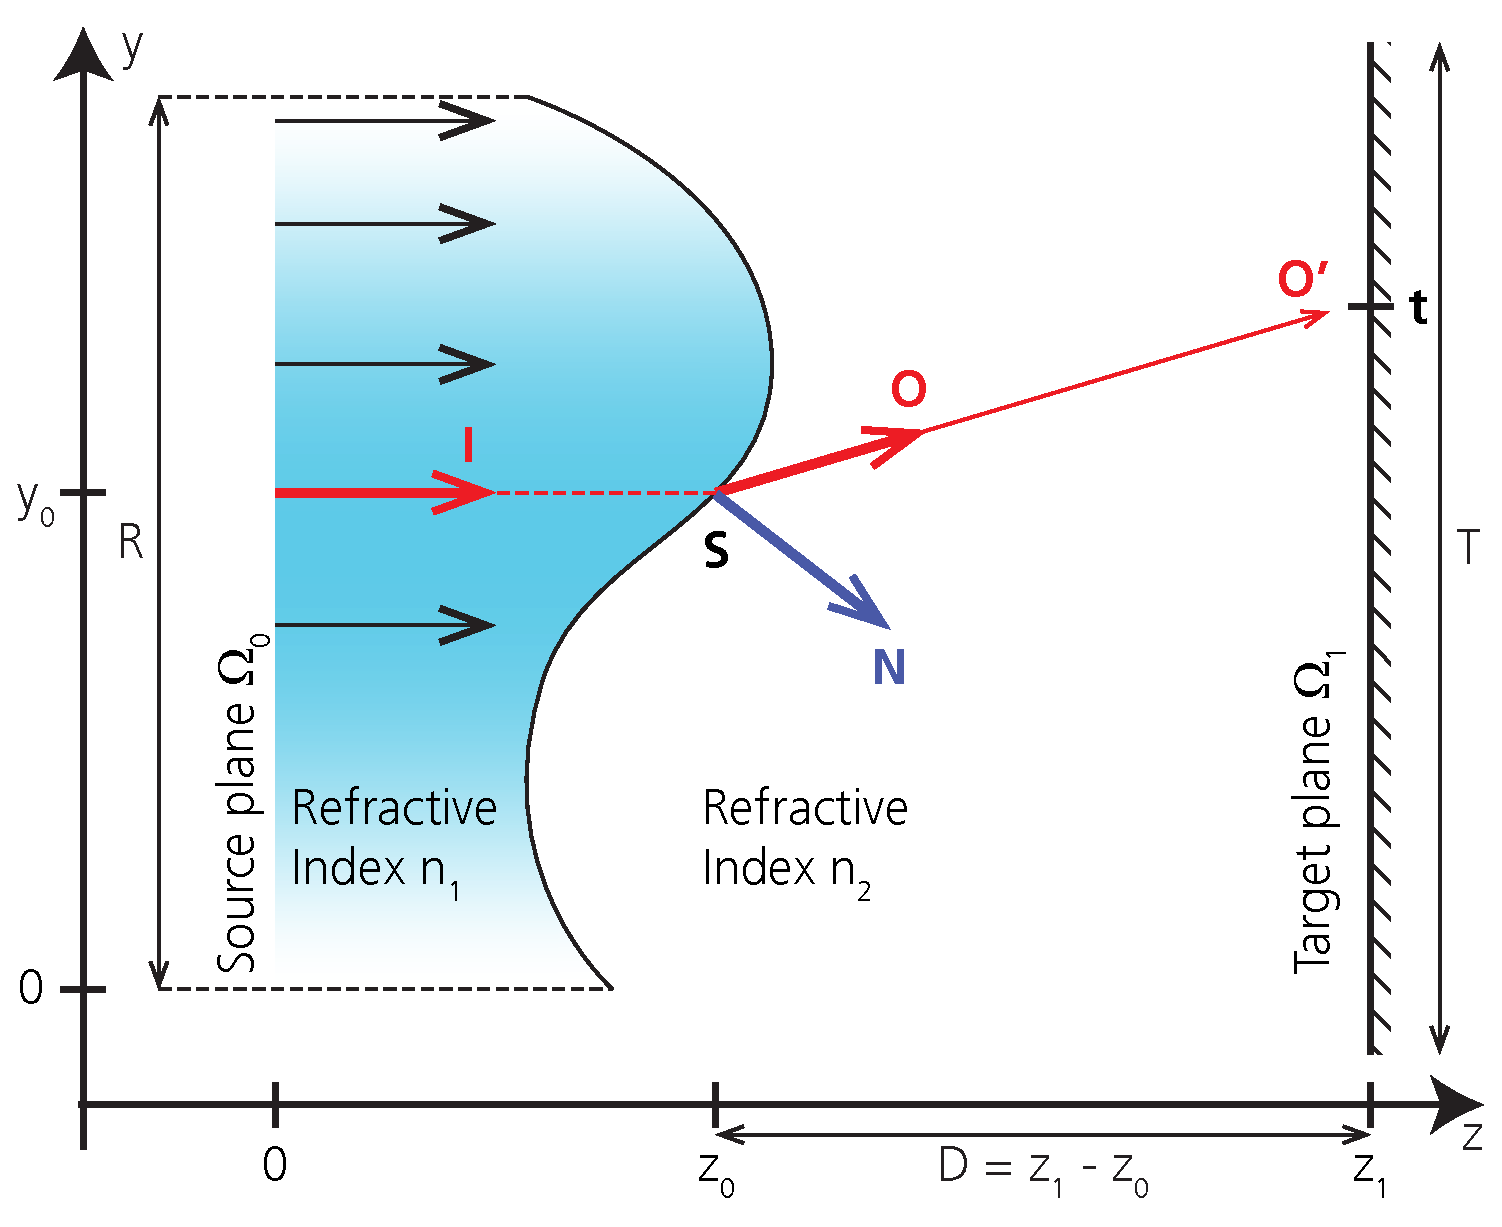
\includegraphics[width=0.49\textwidth]{geometrie_integ}
  \caption{Single-surface setup with a collimated source.}
  \label{fig:1surf-setup}
\end{figure}

Denoting $\I$ and $\OO$ the light incident and output unit vectors onto 
an optical surface with unit normal $\mathbf{N}$, one can write 
Snell's laws in a vectorial form\cite{Benitez2004b}:
\begin{equation}
  n_1 \mathbf{N} \times \mathbf{I} = n_2 \mathbf{N} \times \mathbf{O} 
  \label{eq:snell}
\end{equation}

From this, it follows that 
\[ \N=\Np\big/ \|\Np \|\text{~with~}\Np = n_1 \I - n_2 \OO,\]
Given a mapping $u$, the set of unit vectors $\I$ and $\OO$  can 
directly be seen as full 3D vector fields (by associating the vector supporting 
the ray to each point along the ray trajectory).
The integrability condition \eqref{eq:integ} applies equally to the non-normalized
vector field $\Np$, which yields:
\[ C = \left( n_1 \I - n_2 \OO \right) \cdot
       \left( n_1 \curl{\I} - n_2 \curl{\OO} \right) \]
This can be expanded into:
\begin{align*}
 C =\quad & n_1^ 2 \I\cdot(\curl{\I}) + n_2^2 \OO\cdot (\curl{\OO}) \nonumber \\
 & - n_1 n_2 ( \I \cdot (\curl{\OO}) + \OO\cdot (\curl{\I}))
\end{align*}

%In the setup considered here,
%the curl of the source rays is null, and hence $\I$ always 
%fulfills~\eqref{eq:integ}. 
Zero-\'{e}tendue ray bundles in homogeneous media (like our source) 
are always irrotational~\cite{Minano2004z}, and hence $\I$ always 
fulfills~\eqref{eq:integ}. 
With an irrotational mapping,
the output field $\OO$ also satisfies the same integrability
condition (see detailed computation below).

This yields a necessary and sufficient condition 
on the input and
output fields for the surface normals $\N$ to fulfill~\eqref{eq:integ},
\begin{eqnarray}
%\I\cdot(\curl{\I}) & = & 0  \label{eq:integI} \\
%\OO\cdot(\curl{\OO}) & = & 0  \label{eq:integO}\\
\I\cdot(\curl{\OO}) & = & 0, 
\label{eq:integIO}
\end{eqnarray}
as the two other terms $\I\cdot(\curl{\I})$ and $\OO\cdot(\curl{\OO})$ 
are null.
Note that the demonstration made here is independent of the coordinate
system and that it can be equally derived for reflectors.

We now show that: a) the output field $\OO$ satisfies the
integrability condition~\eqref{eq:integ} and b) that the left term
in~\eqref{eq:integIO} is the limiting factor for the approximation
in~\cite{Baeuerle2012}. Assuming a Cartesian coordinate system, in
which the target to be illuminated is perpendicular to the optical
axis $z$ (see~Fig.~\ref{fig:1surf-setup}), we consider an arbitrary
point between the source and the target, $\mathbf{S}=(x_0,y_0,z_0)$.
If an optical surface is to be constructed at this point in space, a
unique incoming light ray is associated with it. Such a ray is
uniquely identified as a 2D point $(x_0,y_0)\in\Omega_0$ in the source
projection plane. The mapping prescribes that this light ray be
deflected to hit the target at a point $\mathbf{t}$ with coordinates:
\[ \mathbf{t} = \mathbf{u}(x_0, y_0) + z_1 \mathbf{e}_z \]
with $z_1$ as the (fixed) coordinate of the target plane along the $z$
axis, $\mathbf{e}_i$ as the unit vector along direction $i$ and $\mathbf{u}$
having a null $z$ coordinate.  The
non-normalized outgoing direction after refraction is then:
\[  \Op =  \mathbf{t} - \mathbf{S} = 
          \mathbf{u}(x_0, y_0) - x_0\,\mathbf{e}_x -y_0\,\mathbf{e}_y +
          (z_1-z_0) \mathbf{e}_z \] 
This whole expression is irrotational if the mapping's curl itself is
null (due to the linearity of the curl).  It follows that the
normalized output direction $\OO = \Op / \|\Op\| $ satisfies the
integrability condition (\ref{eq:integ}).
The left term of~\eqref{eq:integIO} becomes (see appendix for the 
expansion of the first curl):
\begin{align*}
\I\cdot(\curl{\OO}) & = \I \cdot \left(-\Op\times
\grad{\frac{1}{\|\Op\|}}\right) \\ 
& = \I \cdot \left(\Op\times \frac{\Op \times (\curl{\Op}) +
  (\Op\cdot\grad{})\Op} {\|\Op\|^3} \right) \\ 
&= - (\Op \times \I).\frac{(\Op\cdot\grad{})\Op}{\|\Op\|^3} \\
&= - (\OO \times \I).\frac{(\OO\cdot\grad{})\Op}{\|\Op\|} \\
\end{align*}
The gradient of $\OO'$ expresses the variation of the light output
direction when moving along the optical surface.  In a first order
approximation (the projection-gradient operator $\OO\cdot\grad{}$
being held constant) it has a norm which is of the order of magnitude
of the target size $T$ divided by the optics size $R$. The norm
$\|\Op\|$ has the order of magnitude $D=z_1-z_0$, i.e. the distance
between the surface and the target.  The whole expression is hence
locally proportional to:
\begin{eqnarray}
 C \propto \frac{T}{RD} 
 \label{eq:map_quality}
\end{eqnarray}
Thus the quality of the mapping procedure increases \emph{linearly}
with the reduction of this ratio, that is to say, either by increasing
the distance to the target $D$, by increasing the size of the optic
$R$, or by decreasing the size of the target $T$. Note that this final
term still has the dimension of the inverse of a length, which is
consistent with \eqref{eq:integ}. Also note that this provides only a
local estimate since the projection-gradient operator is not constant
in the general case.

\subsubsection*{Numerical results}
\begin{table*}%[!htbp]
\centering
\begin{tabular}{cc|c|c||c|c|c|}
%\cline{2-7}
% &  \multicolumn{6}{|c|}{Integrability condition ($\times 10^{-5}\,mm^{-1}$)} \\
  \cline{2-7}
\multicolumn{1}{c|}{} & \multicolumn{3}{c||}{Max} & \multicolumn{3}{c|}{RMS} \\ 
\cline{2-7}
\multicolumn{1}{c|}{} & 1/T & R & D & 1/T & R & D \\  \cline{2-7}
\hline 
\multicolumn{1}{|c|}{No mapping optimization} & \multicolumn{3}{c||}{3770} & 
\multicolumn{3}{c|}{733} \\ 
\hline 
\multicolumn{1}{|c|}{Optimized mapping} & \multicolumn{3}{c||}{70.7} & 
\multicolumn{3}{c|}{10.9} \\ 
\hline 
\multicolumn{1}{|c|}{Parameter $\times 2$} & 19.8 &  23.6 & 22.6 & 2.83 & 3.22 & 3.06 \\ 
\hline 
\multicolumn{1}{|c|}{Parameter $\times 4$} & 9.28 &  9.24 & 9.72 & 1.39 & 1.37  &  1.40 \\ 
\hline 
\end{tabular}
\caption{Residual curl of the surface normal field for various geometrical configurations, in units of $10^{-5}\mathrm{~mm^{-1}}$}
\label{tab:map}
\end{table*} 

To validate the approximation given by Eq.~\eqref{eq:map_quality}, a
sample configuration with a square collimated source illuminating a
single-surface lens similar to Fig.~\ref{fig:1surf-setup} was set
up. The initial optics size is $R=50\mathrm{~mm}$, the initial target
position is $D=1000\mathrm{~mm}$ and the initial target size is
$T=200\mathrm{~mm}$. The source provides homogeneous illuminance of
the surface and the target irradiance is a complex pattern (rendering
of the letter ``B'', see Fig.~\ref{fig:letterb}).

\begin{figure}[!htbp]
  \centering 
  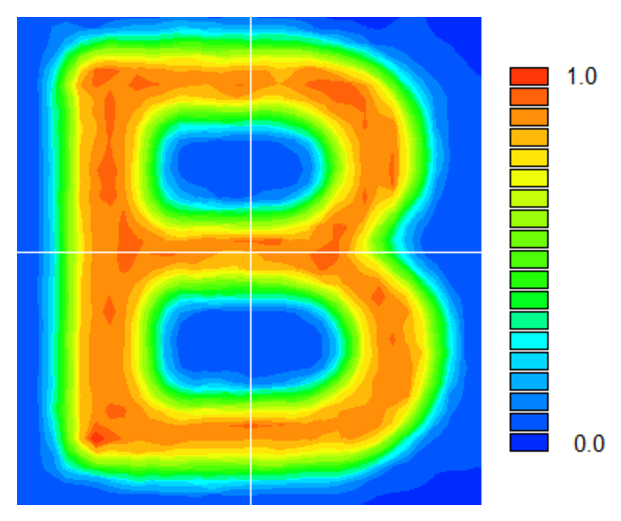
\includegraphics[width=0.35\textwidth]{app_letter_crop}
  \caption{Irradiance pattern as found by ray tracing for the case of
    an irrotational mapping}
  \label{fig:letterb}
\end{figure}

The integrability condition Eq.~\eqref{eq:integ} is computed with a
standard central difference scheme on a 3D discrete grid ($50\times 50
\times 3$ points) located in a $(x,y)$-plane close to the source
($z=10\mathrm{~mm}$) and with a vertical extent equal to the optics
size. Table~\ref{tab:map} shows the maximum absolute value and the RMS
of the curl for various configurations where one of the three parameters
$(1/T), R$ and $D$ has been progressively scaled up, the two others being 
held constant. All values are
given to three significant digits. The first line shows the value of
the curl using the initial values of the three parameters and a
non-optimized ray mapping (i.e. the starting mapping which still has a
significant curl). The second line corresponds to the initial value of
the geometrical parameters, but this time with the irrotational
mapping found using Eq.~\ref{eq:haker-ev}.  The improvement observed
(factor of about~60) confirms that the removal of the mapping's curl
provides a better adherence to the integrability condition
Eq.~\eqref{eq:integ}.  Finally, the three parameters are multiplied by
two (respectively four) and a corresponding reduction by a factor well
over two (respectively four) can be seen in the integrability
condition. This confirms the locally linear behavior expressed
in~\eqref{eq:map_quality}.


\subsection{Point source case}

In the case of a source point what follows shows that the reasoning still holds for  
small source emission angles only (which could also directly be stated
arguing  that this is close to the collimated case).
We don't see yet a broader generalization.

\begin{figure}[!htbp]
  \centering 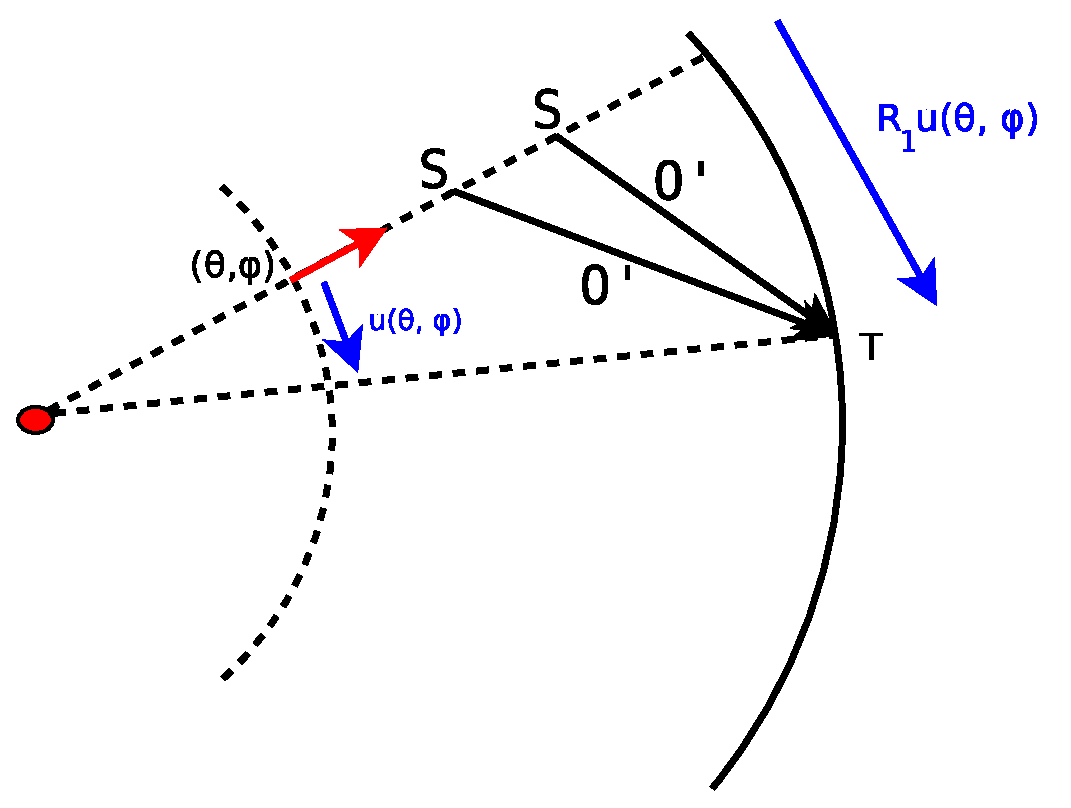
\includegraphics[width=0.45\textwidth]{appendix_sph}
  \caption{Point source configuration with a spherical
  coordinates parametrization. A ray is uniquely determined by the two angles $(\theta, \phi)$.  
  }
  \label{fig:appendix_sph}
\end{figure}


We switch to spherical coordinates.
The direct equivalent of the previous mapping is a function between
 two unit spheres (for example with $R=1$). That
is to say:
\[ \mathbf{A} : (\theta,\phi) \mapsto (t_\theta, t_\phi)\]

%To be able to apply Haker's equation, those two unit spheres are projected 
%in the code onto two planes $\Omega_0$ and $\Omega_1$ with a given projection
% $\mathbf{p}$
%(typically at present, a stereographic projection):
%\[ \mathbf{p}: (\theta, \phi) \mapsto (\rho, \phi)\]
%with $(\rho, \phi)$ the polar parametrization of the plane.
%
%For an arbitrary point $\s(\theta, \phi, r)$ in between the source and the target sphere,
%the point to be reached according to mapping is then:
%\[ T(\theta, \phi, R_1) = R_1 \mathbf{\tilde{u}}(\theta, \phi) + R_1 \mathbf{e}_r\]
%with $R_1$ the fixed radius of the target sphere (note the multiplication by $R_1$
%this time to account for the  bigger radius of the target).
%Consequently:
%\[ \Op = \T - \s = R_1\mathbf{\tilde{u}}(\theta, \phi) + (R_1-r)  \mathbf{e}_r\]
%or equivalently:
%\[ \Op = \T - \s = R_1\mathbf{p}^{-1}\left[ \mathbf{{u}} (\mathbf{p}(\theta, \phi)) \right]
% + (R_1-r)  \mathbf{e}_r\]
%
%With a spherical parametrization a point $\s(r, \theta, \phi)$ in 3D is associated
%uniquely to a point in a plane $\tilde{\s}$ with polar coordinates $\tilde{\s}(p(\theta), \phi)$.
%We assume indeed that the projection from the unit sphere to the plane conserves
%the azimuthal angle.

On the other side the 2D Haker's mapping writes with a polar parametrization:
\[ \mathbf{u}: (\rho, \phi) \mapsto (u_\rho(\rho, \phi), u_\phi(\rho, \phi)) \]
where $\rho$ is the polar radius and $\phi$ the polar angle.
This 2D function is once again made irrotational (with the same procedure)
 which in polar coordinates means (see Appendix):
\[ u_\phi + \rho\pderiv{u_\phi}{\rho} - \pderiv{u_\rho}{\phi} = 0 \]

The link between $\mathbf{u}$ and $\mathbf{A}$ is the projection from the 
unit sphere into the plane. We assume this projection to be rotation symmetric and hence
we write:
\[ p :\theta  \mapsto \rho \]

If the target is a sphere located at $r=R_1$ the light has to reach the point:
\[ \T(R_1, \theta, \phi) = R_1 \mathbf{A}(\theta, \phi) + R_1\mathbf{e}_r \]
with the field $\mathbf{A}$ being the mapping field linked to the 2D Haker's field
by the following relationships:
\begin{eqnarray*}
A_r &=& 0  \\
A_\theta &=& q[u_\rho(p(\theta),  \phi)]  =  q[u_\rho(\p)]  \\
A_\phi &=& u_\phi(p(\theta),  \phi)  = u_\phi(\p)
\end{eqnarray*}
where $p$ is the rotation-symmetric 
projection mentioned above,
and $q$ is its inverse. Furthermore $\p$ is
the projected point in the Haker's plane with radial coordinates
$ (\rho, \phi) = (p(\theta), \phi)$.

As for the collimated case the non-normalized field $\Op$ is still written:
\[ \Op = \T - \s \]
and computing the curl of $\Op$ amouts to compute the curl of $\mathbf{A}$.
We will need the following partial derivatives:
\begin{eqnarray*}
\pderiv{A_\phi}{\theta} &=& p'(\theta)\pderiv{u_\phi}{\rho}(\p)\\
\pderiv{A_\theta}{\phi} &=& \pderiv{u_\rho}{\phi}(\p)q'[u_\rho(\p)] 
\end{eqnarray*}

The formula of the curl in spherical coordinates (see appendix) result in
the following angular curl components:
\begin{eqnarray*}
C_\theta &=& -A_\phi / r = -u_\phi(\p) /r \\
C_\phi &=& A_\theta /r  = q[u_\rho(\p)] /r
\end{eqnarray*}

The last term of the curl along the radial direction is the tricky one:
\begin{eqnarray*}
C_r &=& \frac{1}{r\sin(\theta)} \left[ \sin(\theta) \pderiv{A_\phi}{\theta} +
   \cos(\theta) A_\phi - \pderiv{A_\theta}{\phi} \right] \\
& =& \frac{1}{r\sin(\theta)} \left[ \sin(\theta) p'(\theta)\pderiv{u_\phi}{\rho}(\p)
    + \cos(\theta) u_\phi(\p) - \pderiv{u_\rho}{\phi}(\p)q'[u_\rho(\p)] \right]  \\
\end{eqnarray*}

Assuming that: (a) $\theta$ remains small enough, and (b) that $p$ is such that its 
derivative close to the origin is equal to one (this last assumption is
not very strong and easy to satisfy), we can write:
\begin{eqnarray*}
\sin\theta &\simeq \theta \\
\cos\theta &\simeq 1 \\
p'(\theta) = q'[u_\rho(\p)] &\simeq 1
\end{eqnarray*}
hence leading to:
\[ C_r \simeq \frac{1}{r\sin(\theta)} \left[ \rho \pderiv{u_\phi}{\rho}(\p)
    +  u_\phi(\p) - \pderiv{u_\rho}{\phi}(\p) \right]  \simeq 0\]

If this last term is considered null, the curl of $\Op$ is perpendicular to $\I$
(it has only ortho-radial components) and
the same computation as before can be performed.

%We know that the curl of $\mathbf{u}(\rho, \phi)$ is null (Haker), but it is far
%from obvious that this holds when composing with~$\mathbf{p}$ and its inverse.

%However if $p =\, $Id, the reasoning should still hold (\red{TBC numerically - Adrien}).
%The limiting term would then write:
%\[ C \propto \frac{T_\theta}{R_\theta Z}\]
%with $T_\theta$ the \textit{angular} extent of the target (as seen from the source)
%and $R_\theta$ the \textit{angular} extent of the optics (typically $\theta_{max}$
%in the code).
%The limiting term remains locally approximated by:
%\[ C \propto \frac{T}{R Z}\]


%\textbf{TODO: if this is is correct, this would mean the stereographic 
%projection is to be reviewed - we should perform
%a much more simple projection: $(\theta, \phi) \mapsto (r = \theta, \phi)$. 
%\red{Wrong} - we simply need a projection which is linear at the origin
%}
%
%Numerical results computed with this projection: see table \ref{tab:map_point}

%\begin{table*}[!htbp]
%\centering
%\begin{tabular}{cc|c|c||c|c|c|}
%\cline{2-7}
% &  \multicolumn{6}{|c|}{Integrability condition ($\times 10^{-3}\,mm^{-1}$)} \\
%  \cline{2-7}
%\multicolumn{1}{c|}{} & \multicolumn{3}{c||}{Max} & \multicolumn{3}{c|}{RMS} \\ 
%\cline{2-7}
%\multicolumn{1}{c|}{} & 1/T & R & Z & 1/T & R & Z \\  \cline{2-7}
%\hline 
%\multicolumn{1}{|c|}{No mapping optimization} & \multicolumn{3}{c||}{657} & 
%\multicolumn{3}{c|}{205} \\ 
%\hline 
%\multicolumn{1}{|c|}{Optimized mapping} & \multicolumn{3}{c||}{20.6} & 
%\multicolumn{3}{c|}{4.94} \\ 
%\hline 
%\multicolumn{1}{|c|}{Parameter +25\%} & 12.1 &  10.4 & 12.0  & 3.26 & 3.32 & 3.20 \\ 
%\hline 
%\multicolumn{1}{|c|}{Parameter +50\%} & 9.96 &  7.64 & 9.40 & 3.16 & 2.57  &  2.88 \\ 
%\hline 
%\end{tabular}
%\caption{Integrability condition for various geometrical configurations in a point source run}
%\label{tab:map_point}
%\end{table*} 
%
%Doesn't hold when scaling the parameters by $\times 2$ or $\times 4$, confirming
%the local aspect of the ratio given previously.
%However we still observe that the linear estimation is a conservative one.
%\red{wrong interpretation after what precedes ...}

\subsection{General case}

errr ? still relevant ? we virtually handled all null étendue sources

\subsection{Multiple freeform surfaces}

tough one




\section{Flux optimization}
\subsection{Light flux propagation}

Taking a different approach, we now propose an extended algorithm that
allows to significantly improve the initial design resulting from the
optimized mapping derived in the previous section and allows to design
multiple optical surfaces.  Assuming as in the previous section that
the optical surface is represented as a three-dimensional triangular
mesh, each node of the mesh constituting the first surface has its
position determined by the direction of a source ray (a unit vector),
multiplied by a scalar value. Those directions are held constant
during the construction of the surfaces (only the scalar factors are
varied).

\begin{figure}[!htbp]
  \centering 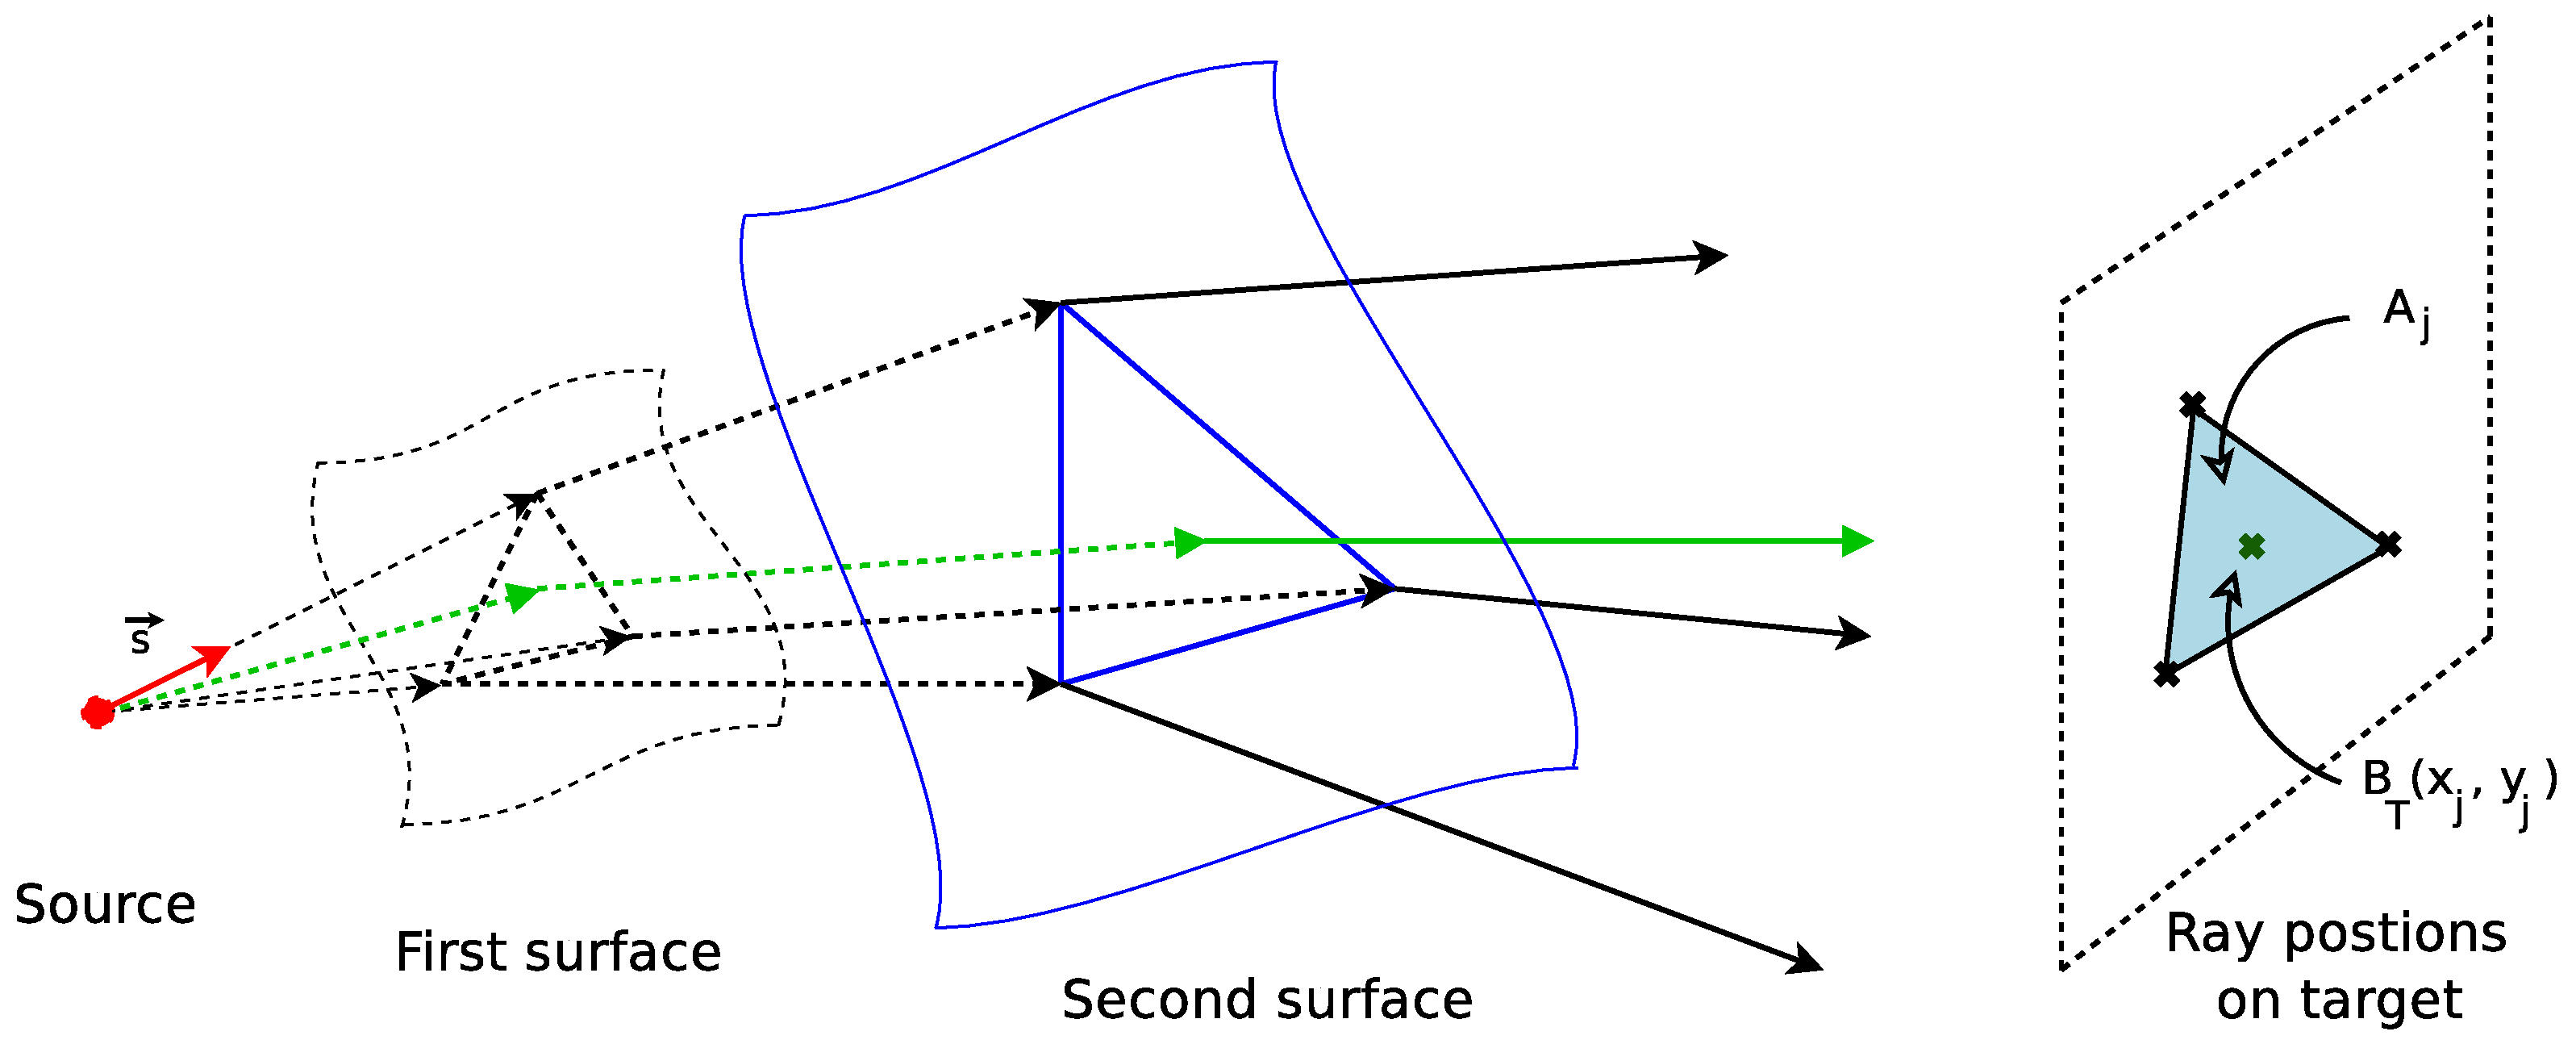
\includegraphics[width=0.9\textwidth]{rays_new}
  \caption{Elementary light flux tube (prism-shaped) delimited by the rays passing
    through the vertices of a triangular surface element (blue). The
    vertex rays are represented in dark, the face ray in green.  If
    the vertex ray \textit{directions} (e.g. the red vector
    $\mathbf{s}$) drawn from the source are held constant, the light
    flux within the triangular tube also remains constant.}
  \label{fig:rays}
\end{figure}


We observe that, on the one hand, the flux emitted by the source
$\Phi_S$ can be written as follows:
\begin{itemize}
\item for a point source:
  \begin{equation}
   \Phi_S = \iint d^2\Phi_S = \iint I(\theta, \phi) d^2\Omega
   \label{eq:flux_src_point}
  \end{equation}
  where $d^2\Phi_S$ is the elementary light flux, $d^2\Omega$ the
  elementary solid angle surrounding the direction of emission
  $(\theta, \phi)$, and $I(\theta, \phi)$ is the radiant intensity (in
  $\mathrm{W/sr}$) of the point source.  The elementary solid angle
  $d^2\Omega$ is approximated by the solid angle encompassed by the
  three source rays around a triangular face
  (see~Fig.~\ref{fig:rays}).  This solid angle remains constant
  throughout the construction.

\item for a collimated source:
  \begin{equation}
   \Phi_S = \iint d^2\Phi_S = \iint B_S(x, y) dx\,dy 
   \label{eq:flux_src_coll}
  \end{equation}
  where $B_S(x,y)$ is the source (radiant) irradiance (in $\mathrm{W/m^2}$).  In
  this case, the source rays are all directed towards the
  same direction (e.g. along the $z$-axis) and the cross section of a
  triangular tube remains constant between the source and the first
  optical surface.
\end{itemize}
In both cases, the flux from the source within a triangular tube
remains constant along its path through the optical system,
 as illustrated by Fig.~\ref{fig:rays}.

On the other hand, the flux reaching the target $\Phi_T$ can be
written as a function of the irradiance (in $\mathrm{W/m^2}$) on the target.  A
triangular flux tube is projected as a triangular area on the target
as illustrated in Fig.~\ref{fig:rays}.  The flux in this tube can be
computed as:
\[ \Phi_T(j) = \iint_{A_j} B_T(x, y) dx\,dy \]
where $A_j$ is the area of the target triangle corresponding to the
$j$-th face of the surface, and $B_T(x,y)$ the desired irradiance at
the target point $(x,y)$. This integral is approximated with the
simplest quadrature:
\begin{equation}
  \Phi_T(j) = B_T(x_j, y_j) A_j
  \label{eq:flux_target}
\end{equation}  
with $(x_j, y_j)$ being the center of the triangular face on the
target as illustrated in~Fig.~\ref{fig:rays}.


\subsection{Smoothing terms}

\subsubsection{Objective function components}
Similarly to the purely mapping-based approach in~\cite{Baeuerle2012},
a least-squares optimization procedure is proposed. Taking into
account the description of the light flux above, the merit function
being optimized can now be detailed as a collection of three
components:

\begin{itemize}
\item{\emph{light flux difference}}: this component aims to equalize
  the light flux in Eqs.~\eqref{eq:flux_src_point} (or
  \eqref{eq:flux_src_coll}) and~\eqref{eq:flux_target}. It ensures
  that the desired irradiance $B_T(x, y)$ is achieved on the target;
\item{\emph{smoothing component}}: in order to avoid local minima
  corresponding to triangular mesh components with abnormally high or
  low radiant intensity values (distorted triangles), a smoothing component is
  added. It enforces that face rays intersect the target near the
  center of the respective triangular area on the target. 
  A face ray is closely correlated to the normal vector of the 
  corresponding triangular face on the optical surface. Thus this 
  component gives the advantage to nearly co-planar neighbor triangles 
  on the optical surface;
\item{\emph{distance to target's boundary}}: the source and the target
  total light flux are both normalized to unity, so that all the
  source rays going through the system must eventually reach the
  target. This is explicitly enforced by penalizing edge rays which
  deviate too far from the target boundary.
\end{itemize}

\subsubsection{Numerical considerations}
A consistent and homogeneous scaling of the three merit function
components allows a better numerical stability, the ability to easily
scale up or down the resolution of the surface (number of triangles),
or the possibility to change the geometry of the problem without
re-adjusting from scratch the convergence criteria of the optimizer.

All three components of the objective function above are hence chosen
to be homogeneous to unity and to remain of the same order of
magnitude, regardless of the geometry or resolution of the problem:
\begin{itemize}
\item the flux difference for a face is multiplied by the number of
  faces.  Since the source flux is already normalized to unity, this
  ensures the scalability with regards to the number of triangles in
  the mesh. The effective light flux going through a face hence always
  has the order of magnitude unity;
\item the smoothing component is scaled by the typical size of a
  triangle area on the target which varies as the square root of the
  total number of triangles;
\item the distance to the target boundary is scaled by the target
  size.
\end{itemize}

The optimization procedure also involves the computation of a
numerical gradient in the form of a standard forward difference using
a step size $h$. It can be shown\cite{Bindel2009} that on a
finite-precision machine with machine precision $\epsilon_m$ such a
computation leads to the following final relative error:
\begin{equation}
 \tilde{f'}(x) = f'(x) \left(1 + \epsilon_m \frac{2f(x)}{hf'(x)} +
 \frac{f''(x)}{2f'(x)}h \right)
 \label{eq:grad_error}
\end{equation}
with $\tilde{f'}(x)$ the numerical approximation of the derivative and
$\epsilon_m$ the machine round-off precision.  The last two terms are
competing one with another and dictate an optimal value for $h$.
Noting $\epsilon_m = 10^m$, $h = 10^n$, ${2f}/(hf') = 10^u$ and
${f''(x)}/(2f'(x)) = 10^v$ the optimal value of $n$ satisfies $ v+n =
-n+u+m $, hence:
\[n = (u-v+m)/2\]
Typically, with the scaling considerations mentioned above $(u,v,m) =
(-1, -1, -15)$ giving a step size $h \approx 10^{-7}$ and an overall
relative computation precision around $\epsilon = 10^{v+n} \approx
10^{-8}$.  However the computation above discards the error induced by
the evaluation of $f$ itself (propagation error): a slightly bigger
step size (around $h \approx 10^{-6}$) gives in practice better
results and has been retained in the final implementation.

Finally, the computation time using this new objective function is
about a factor 4 longer than the mapping-only approach, but this remains 
within minutes on a standard PC for typical applications (general lighting,
automotive, etc ...).

\section{Sample applications}
\label{sec:results}
The procedure presented above allows the design of various optical
configurations with a wide range of applications. We present two
complex cases. For each design below the improvement between the
initial mapping approach and the flux optimized approach is presented,
and the examples are given in order of increasing difficulty.

\subsection{Double sided freeform lens}
First, a refractive case with two freeform surfaces is presented.  The
target plane is positioned perpendicular to the light axis and is
centered on it at a distance of $100\mathrm{~mm}$.  The prescribed irradiance
is the letter~``B''.

\begin{figure}[!htbp]
  \centering \includegraphics[width=1.0\textwidth]{app-B}
  \caption{Double sided freeform lens projecting the letter ``B''
    (lengths in~$\rm mm$, irradiance in~$\rm a.u.$); (a) with mapping
    optimization only; (b) with mapping and flux optimization; (c)
    lens CAD model, the source is positioned at the origin of the
    coordinate system.  }
  \label{fig:letter}
\end{figure}

The flux optimization provides a sharper cut-off at the boundaries of
the pattern as can be seen in the two middle holes, and on the upper
and lower tips of the left part of the distribution.  The two freeform
surfaces forming the lens were designed using 4,000 triangles for each
optical element.  The final surfaces consist of two NURBS fitted to
the two triangular meshes.  The design assumes that the lens is made
of glass ($n=1.5$) and that a light cone with a half-angle of
45~degrees is captured from the point source.
%%% CONFLICTING with what Loo said, but I prefer Reviewer 1's comment:
%The resulting optical efficiency amounts to 46\%
%(including Fresnel losses).

\subsection{Logo lens}
To demonstrate the abilities of the presented algorithm a much more
elaborate example is presented.  The optics has been designed for a
perfectly collimated source. The logo is projected on a surface of $55
\times 17.5\,mm^2$ at a distance of $100\,mm$ from the source, and has
a resolution of $530 \times 160$~pixels. We present the results with
one and two freeform surfaces, respectively. The optics has a size
close to the target one: $50 \times 15\,mm^2$.

\begin{figure}[!htbp]
  \centering 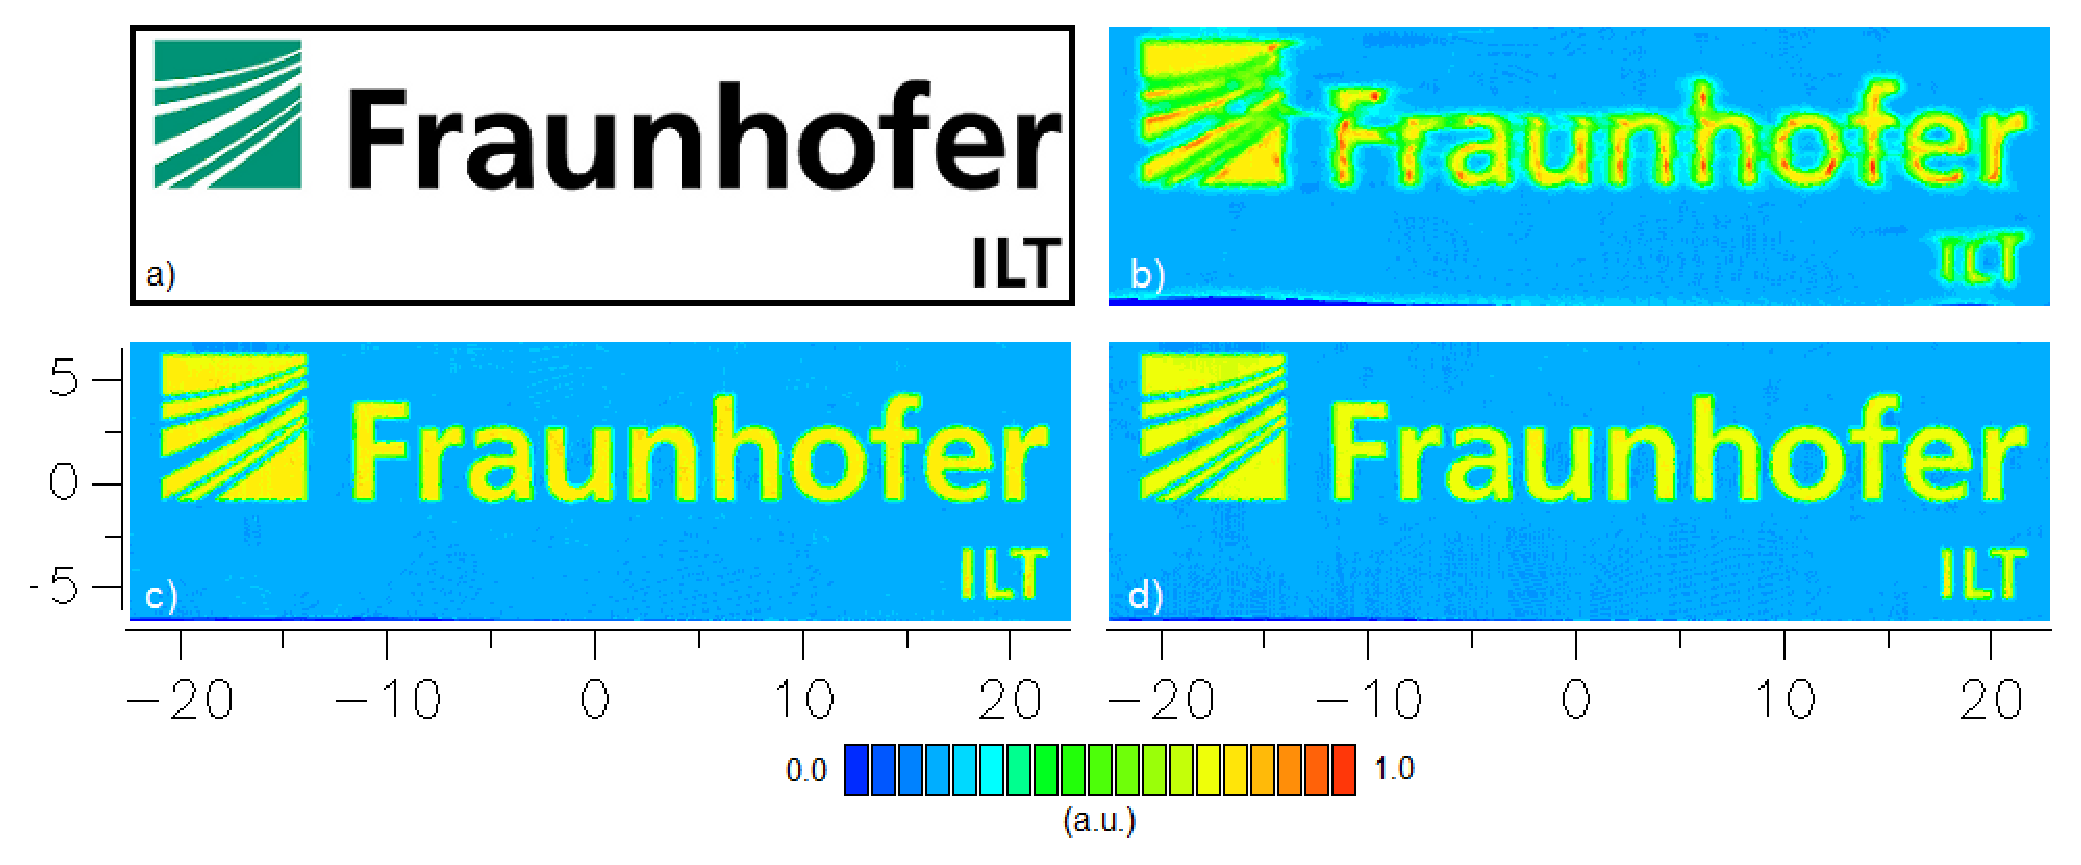
\includegraphics[width=1.0\textwidth]{logo_bottom}
  \caption{Ray-tracing of high-resolution logo generated with 16
    million rays (lengths in~$\rm mm$, irradiance in~$\rm a.u.$); (a)
    prescribed irradiance distribution (passed to the algorithm in
    black and white); (b) one freeform surface with mapping
    optimization only; (c) one freeform surface with mapping and flux
    optimization; (d) two freeform surfaces with mapping and flux
    optimization.}
  
  \label{fig:logo}
\end{figure}

The ray tracings presented in Fig.~\ref{fig:logo} were performed with
16~million rays and a detector grid having the same resolution as the
prescribed irradiance.  Once again, the improvement over the mapping
optimization is clearly visible: the contours of the letters making
the logo are much sharper and better defined, particularly in the
bottom right part (see analysis focused on the ``ILT'' part
below). The overall result looks equally satisfactory with one or two
freeform surfaces.

Similar to what has been done previously by Bortz and
Shatz~\cite{Bortz2007}, the following fractional RMS measure was
computed to assess the quality of the design:
\begin{equation}
  RMS= \sqrt{\sum\left(\frac{I_c - I_p}{I_{ref}}\right)^2}
  \label{eq:rms}
\end{equation} 
where $I_c$ is the computed irradiance as given by the ray tracing,
$I_p$ is the prescribed irradiance and $I_{ref}$ is a reference
irradiance.  Bortz and Shatz restricted their computation to an area
where the irradiance was sufficiently high and hence took
$I_{ref} = I_p$.  In our case, given the contrast at hand (about 4:1)
and the fact that the analysis should not be restrained to the letter
cores (areas of high irradiance), we computed the RMS with both
$I_{ref} = I_{avg}$, the (arithmetical) average of the light
irradiance, and $I_{ref} = I_{max}$, the peak irradiance found at the
core of a letter, for example.

For statistical relevance, the analysis was also restrained on a
sub-part of the logo where a fine level of details is found
(see~Fig.~\ref{fig:logo_zoom}).  The sub-area was traced with
2~million rays and covers $66\times39$~detector pixels.  With this
setup the ray tracing of a homogeneous pattern would result in a
statistical relevance of 3-4\%.

\begin{figure}[!htbp]
  \centering 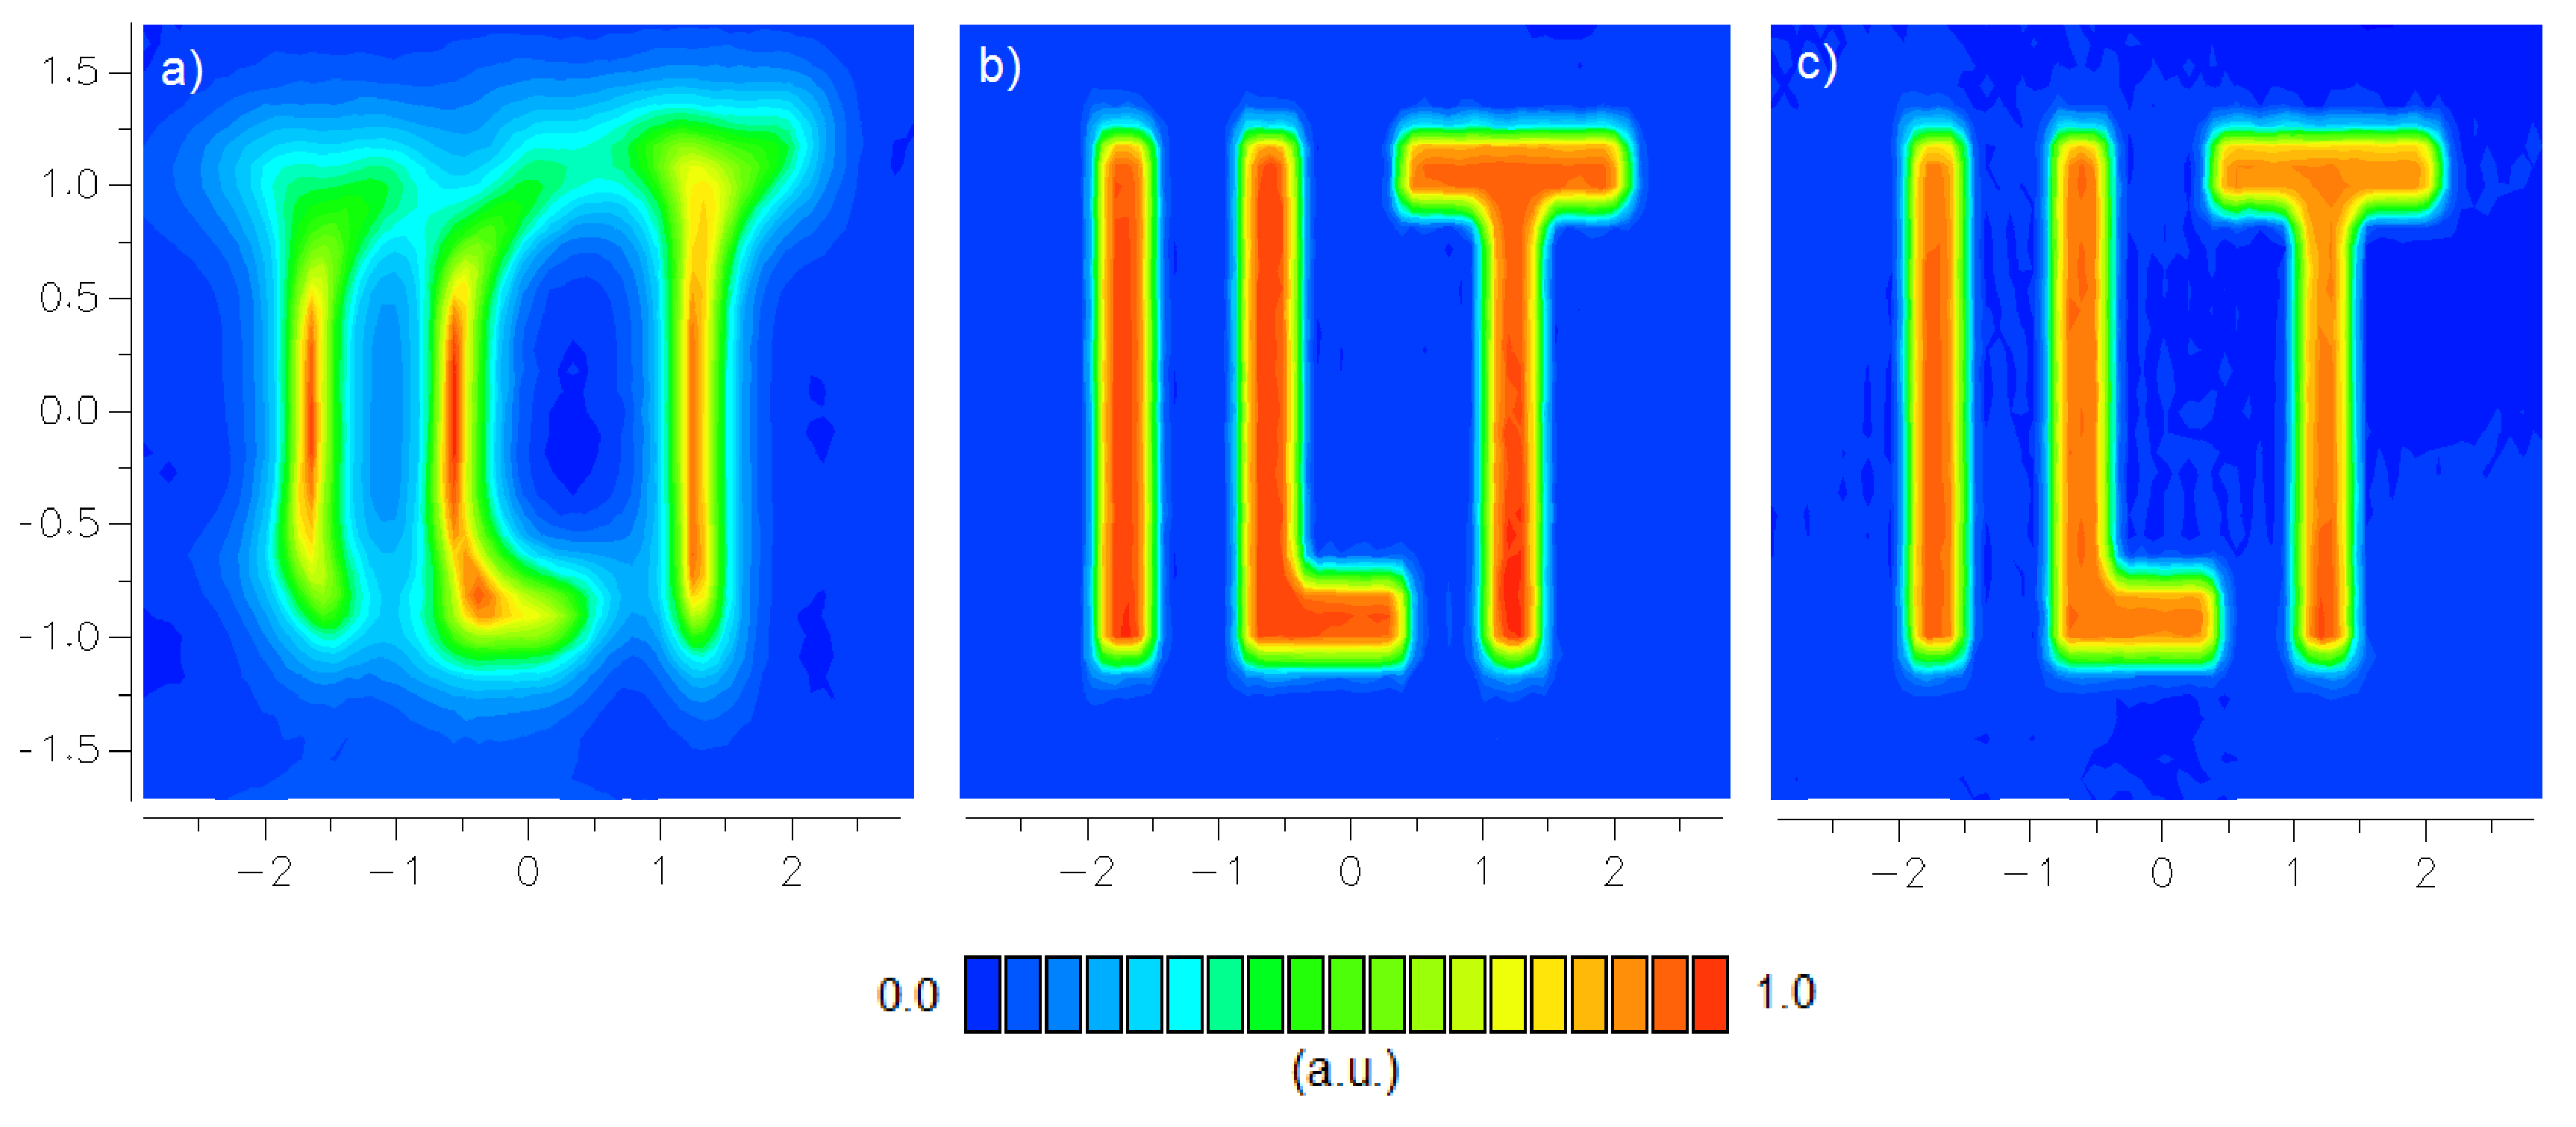
\includegraphics[width=0.95\textwidth]{logo_zoom}
  \caption{Zoom on the lower right part of the logo for RMS
    analysis. Ray-tracing with 2 million rays on a grid of $66 \times 39$
    points (lengths in~$\rm mm$, irradiance in~$\rm a.u.$). 
    (a) one freeform surface with mapping optimization only; 
    (b) one freeform surface with mapping and flux optimization;
    (c) two freeform surfaces with mapping and flux optimization.}
  \label{fig:logo_zoom}
\end{figure}

Table~\ref{tab:rms} presents the resulting fractional RMS computed
with the two different irradiance references (average and maximum).
\begin{table}[!htbp]
  \centering
  \caption{Fractionnal RMS for a sub-area of the logo
    projection. $RMS_{avg}$ (resp. $RMS_{max})$ denotes the RMS
    computed with $I_{ref}$ being the average irradiance (resp. with
    $I_{ref}$ being the peak irradiance)}
  \label{tab:rms}
  \begin{tabular}{c|c|c|}
    \cline{2-3}
      & $RMS_{avg}$ & $RMS_{max}$ \\ \hline
    \multicolumn{1}{|c|}{One surface (mapping optimization only)} 
      & 33.7\% & 16.0\% \\\hline
    \multicolumn{1}{|c|}{One surface (mapping and flux optimization)}
      & 10.1\% & 4.82\% \\\hline 
    \multicolumn{1}{|c|}{Two surfaces (mapping and flux optimization)}
      & 10.2\% & 4.84\% \\\hline
\end{tabular}
\end{table} 
The improvement brought on by the flux optimization is clearly visible for
both references.  The last two lines show that the ray-tracing falls
slightly off the statistical boundary given above. The sharp edges of
the letters forming the logo are challenging to project and prove to
be the main deteriorating factor.  Comparing part b) and c) of
Fig.~\ref{fig:logo_zoom}, we can also identify a slight loss of
irradiance homogeneity within the letters, confirming that the single
surface design is less complicated.  However, in both cases, the shape
of the pattern has clear and well defined contours.

Finally the overall optical efficiency in this case is close to its
maximum theoretical value, since all the rays of the collimated source
are captured by the optical system.




% Extended source 
\chapter{Extended sources}
\label{ch:extended}

\section{Extended source}
\subsection{Two dimensional case - Line source}
Here we consider in 2D a line source perpendicular to the $x$ axis,
and immersed in the refractive medium. 
\subsubsection*{Parametrization}
See the figure \ref{fig:line_src} below.

\begin{figure}[!htbp]
\centering
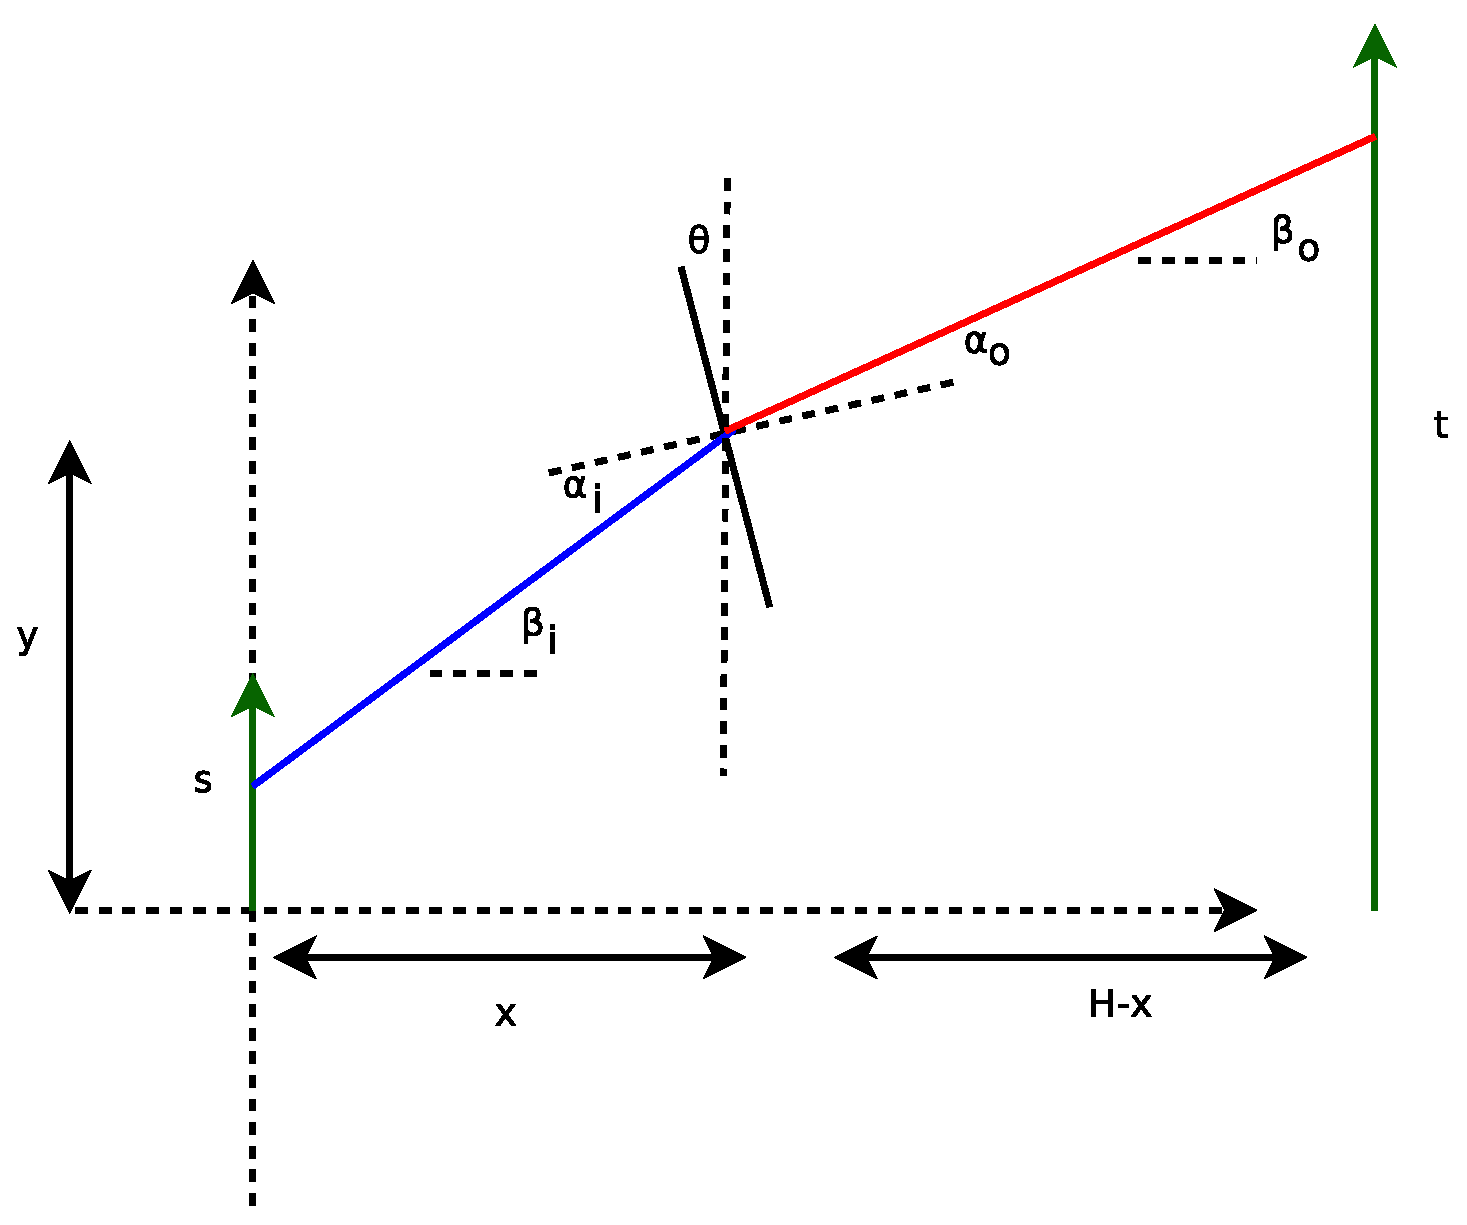
\includegraphics[scale=0.4]{line_src} 
\caption{Parametrization of the extended source setup in 2D.
}
\label{fig:line_src}

\end{figure}


The source line is parametriezd by the coordinate $s$ (along the same
direction as the y axis), the optical surface 
by its curvilinear coordinate $\sigma$, and finally the target
line by the coordinate $t$.
A ray emitted from $s$ to $\sigma$ has an angle $\beta_i$ with 
respect to the horizontal, and similarly a ray from $\sigma$ to
$t$ has an angle $\beta_o$ with the horizontal.
The full source, full optical surface and full target are noted
$S$, $\Sigma$ and $T$ respectively.

It is important to realize that among the 5 variables described so
far ($s,t, \sigma, \beta_i, \beta_o$) we only have two degrees
of freedom. For example, if $t$ and $\sigma$ are given, the other
three variables are completely determined.

\subsubsection*{Light flux conservation}

Physically, the extended source is best described by the concept
of \emph{luminance} (in $cd/m$, or $lm/rad/m$):
\[ L(s, \beta_i) = \frac{d^2\Phi}{ds\,d\beta_i \cos \beta_i}  \]
where $d^2\Phi$ is the elementary light flux (lm), $ds$ the source
surface element, $\beta_i$ the direction of emission and $d\beta_i$
the elementary plane angle in the given direction.
The cosine in the definition was historically introduced to make this
value somewhat independent of the angle of observation 
(a  Lambert emitter has for example a constant \emph{luminance}).
To ease the computation in our case, we will always include 
the cosine in the notation and hence
write:
\[ L_S (s, \beta_i) = \cos\beta_i L(s, \beta_i) \]
for the luminance of the source on any given point 
$s$ on the source plane, and any emission angle
$\beta_i$. $L_S$ remains homogeneous to a luminance in terms of 
physical units.
With this in mind the elementary and the full flux emitted 
from the source are respectively written:
\begin{eqnarray}
\label{eq:elem_src}
 d^2\Phi_S = L_S (s, \beta_i)ds\,d\beta_i \\
 \Phi_S = \iint L_S (s, \beta_i) ds\,d\beta_i
\end{eqnarray}

We now derive the relationship between the source luminance $L_S$
and the \emph{illuminance} $B_T(t)$ (\emph{Beleuchtungstaerke} in $lm/m$) 
on the target. The illuminance is what can be obtained in Fred 
with an ''Analysis Plane'' and is oft the quantity being
optimized.

The elementary flux emitted
from one point of the source, going through one surface point
and reaching one target point is conserved (no energy gain or loss):
\[  d^2\Phi_S = d^2\Phi_T \]

The target illuminance is per definition the light flux for an elementary
target surface element:
\[ d^2\Phi_T = dB_T(\sigma, t)\,dt = A(\sigma, t)\,d\sigma\,dt\] 
The total illuminance at a target point is obtained by summing the contributions
of all the surface elements:
\begin{equation}
 B(t) = \int_\Sigma A(\sigma, t)\,d\sigma
\label{eq:beleuch}
\end{equation}

We now perform two successive changes of variable on the elementary source
flux~Eq.~\eqref{eq:elem_src} to obtain a suitable expression of $A(\sigma, t)$:
\begin{eqnarray*}
d^2\Phi_S &= & L_S(s, \beta_i)ds\,d\beta_i \\
    &      = & L_S(s, \beta_i) \left. \pderiv{s}{\sigma} 
            \right|_{\beta_i=cst} d\sigma\,d\beta_i \\
    &      = & L_S(s, \beta_i)|J_1| \left. \pderiv{\beta_i}{t}
             \right|_{\sigma=cst} d\sigma\,dt \\    
    &      = & L_S(s, \beta_i)|J_1|\,|J_2| d\sigma\,dt \\    
\end{eqnarray*}
with $J_1$ (resp. $J2$) the partial derivatives of $s$ (resp. $\beta_i$) with 
$\beta_i$ (resp. $\sigma$) being held constant (see Appendix) and hence:
\[ A(\sigma, t) =  L_S(s, \beta_i)|J_1|\,|J_2|\]

The first Jacobian $J_1$ could be termed the \textit{face factor}
and expresses how the contribution of each element of the 
optical surface has to be weighted when summing the contributions on the target.
The second Jacobian expresses, for a given surface element,
how the source luminance is turned into an irradiance on the target.

Both computations are detailled further down and gives for Eq.~\eqref{eq:beleuch}:
\[ B_T(t) = \int_\Sigma L_S(s, \beta_i) |J_1| \,|J_2|\, d\sigma \]
Given the internal representation of the optical surface in the 
algorithm, this last integral is approximated as a discrete
sum over the 
elements of the polygonal line constituing the surface:
\begin{equation}
\label{eq:computed_irr}
B_T(t) = \sum_{j \in Faces(\Sigma)} L_S(s_j(t), \beta_{i, j}(t)) 
|J_1| \,|J_2|\,\Delta \sigma_j 
\end{equation} 
where the term $\Delta \sigma_j$ is independent from $t$ and represents the
length of a face.

The whole computation has been validated with FRED ray tracing as illustrated
below on Figure~\ref{fig:fred_ext}.
\begin{figure}
\centering
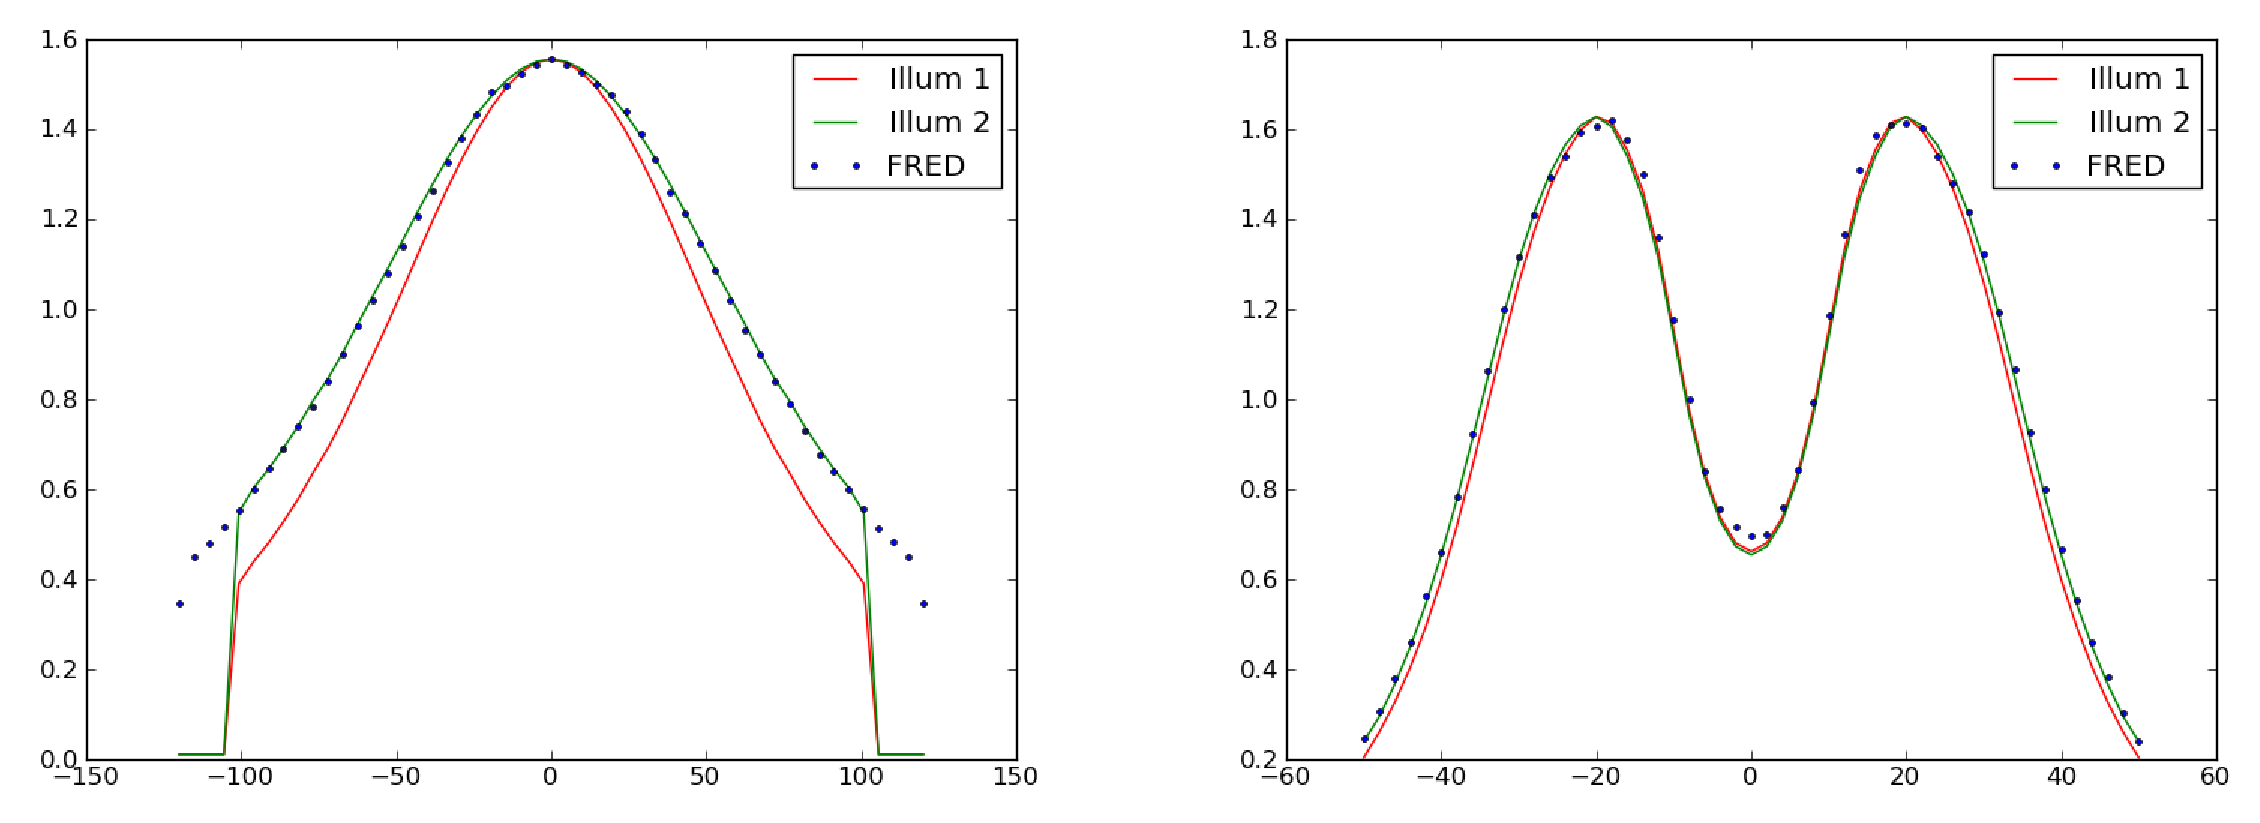
\includegraphics[width=1.0\textwidth]{fred_ext} 
\caption{Ray tracing validation. Left config: shperical surface element (no optim), 50deg.
In red the computed result when neglecting the Jacobian $J_1$. Right config:
after point source optimization. The effect of $J_1$ (still in red)
 is invisible in this case.
 In both cases source is about a third of the optics size.
}
\label{fig:fred_ext}
\end{figure}

\subsubsection*{Face factor - Jacobian $J_1$}
The emittance angle $\beta_i$ is held constant.
The sine law in the triangle plotted on the~Fig.~\ref{fig:ds_dsigma} below writes:
\[ \frac{d\sigma}{\sin\alpha} = \frac{ds}{\sin\beta}\]
with:
\[ \alpha = \pi/2 - \beta_i \quad \quad \beta = \pi - (\theta+\alpha)\]
Hence the first (and final) term of the Jacobian writes:
\[ \pderiv{s}{\sigma} = \frac{\cos(\theta-\beta_i)}{\cos\beta_i} \]

\begin{figure}[!htbp]
\centering
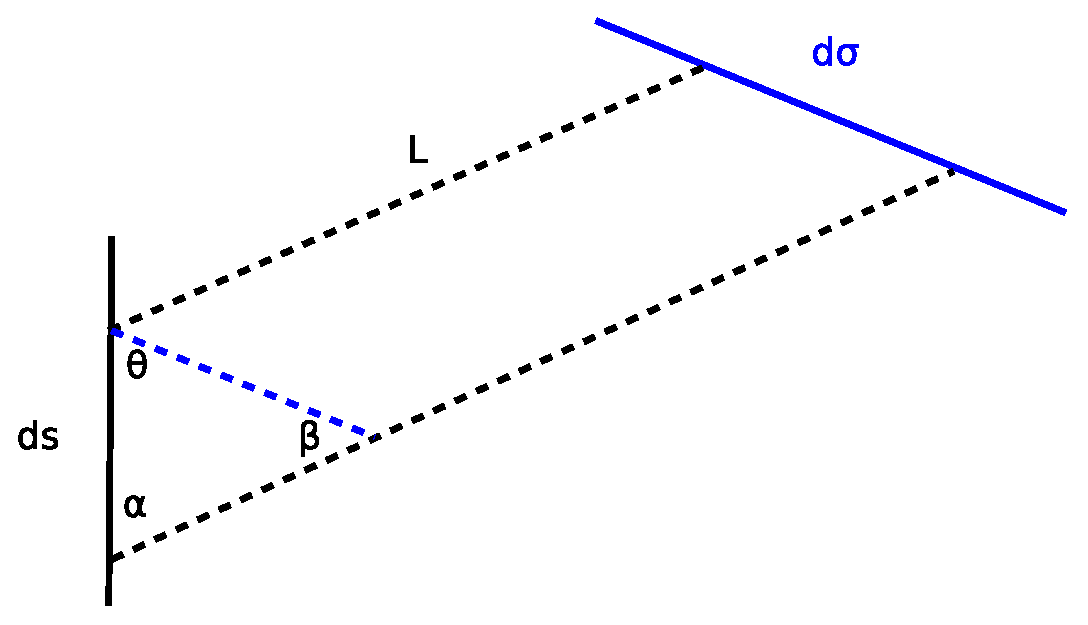
\includegraphics[scale=0.4]{ds_dsigma} 
\caption{Geometric setup for the $J_1$ Jacobian computation. In black
on the left the source plane, in blue on the right, a surface element parametrized
by the curvilinear coordinate $\sigma$. The emittance angle $\beta_i$ is held constant.}
\label{fig:ds_dsigma}
\end{figure}

Note that this factor plays often a minor role, in the sense that it is close
to being constant for small angles.
The figure below shows the corresponding plot in 2D with $\beta_i$ on the X axis
and $\theta$ on the Y axis.

\begin{figure}[!htbp]
\centering
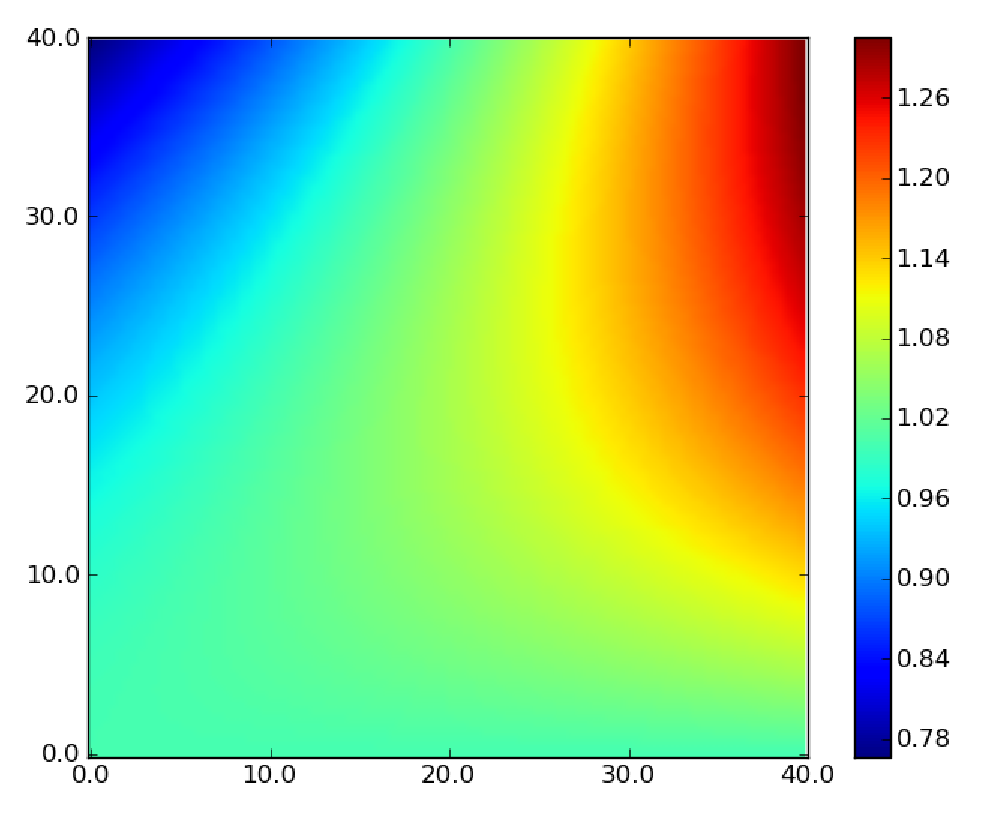
\includegraphics[scale=0.5]{ds_dsigma_jac} 
\caption{Face factor (Jacobian $J_1$). Angle $\beta_i$ on the X axis
and $\theta$ on the Y axis (in degrees).}
\label{fig:ds_dsigma_jac}
\end{figure}


\subsubsection*{Illuminance for an elementary element of the 
optical surface - Jacobian $J_2$}
We compute here the analytical relationship between $s$
and $t$. The computation of the derivative:
\[J_2 = \left. \pderiv{\beta_i}{t} \right|_{\sigma=cst}\]
 will follow naturally.
As mentionned above the computation corresponds to the elementary illuminance
on the target produced by the full source through a small surface
element. This can be tested in FRED taking a (finitely) small plane
to represent an elementary surface element.

We note $\alpha_i$ and $\alpha_o$ the
angles w.r.t. the surface element normal. The surface normal is tilted
by $\theta$ from the horizontal (see figure \ref{fig:line_src}).

Simple geometry then gives:
\[ s = y - x\tan(\beta_i) \]
\[ t = y + (H-x)\tan(\beta_0) \]
and also
\[\beta_i = \theta + \alpha_i \]
\[\beta_o = \theta + \alpha_o \]
and finally from Snell's law:
\[ n \sin\alpha_i = \sin\alpha_o \]
From this one can write:
\[ \beta_i = \theta + \arcsin\left[ \frac{1}{n} 
		\sin(\arctan\frac{t-y}{H-x} - \theta)
 \right]\]

Hence by direct differentiation:
\[ d\beta_i = \frac{\cos(g(t)) }
{ (H-x) \left( 1+(\frac{t-y}{H-x})^2 \right) \sqrt{n^2 - \sin^2(g(t))}} dt\]
with 
\[ g(t) = \arctan\left(\frac{t-y}{H-x}\right) - \theta\]
Substituing the quotient with the above formulas gives an alternative
expression:
\[ g(t) = \arctan\left(\frac{(H-x)\tan\beta_o}{H-x}\right) - \theta = \alpha_o\]
Hence:
\[ d\beta_i = (\cos \alpha_o)
\left[ (H-x) \left( 1+(\frac{t-y}{H-x})^2 \right) \sqrt{n^2 - 
\sin^2 \alpha_o} \right]^{-1} dt\]
%One can then compute $dB_t$ as a function of $t$ (taking for example
%$dI_s(\beta_i) = dI_0 \cos(\beta_i)$ for a uniform Lambert
%emitter).
and:
\[ J_2 = (\cos \alpha_o)
\left[ (H-x) \left( 1+(\frac{t-y}{H-x})^2 \right) \sqrt{n^2 - 
\sin^2 \alpha_o} \right]^{-1} \]


This computation can be avoided by finding a \emph{cubic} 
fit of the coordinate function 
$\beta_i(t)$ (this
requires 4 points marked in green in the example below):
\[ \beta_i(t) = at^3+bt^2+ct +d \]
We then have directly
a \emph{quadratic} fit of the complicated differential:
\[\frac{d\beta_i}{dt}(t) = 3at^2+2bt + c \]

Finally one can also compute the resulting elementary illuminance
produced on the target by an elementary surface element
located at $(x,y)$ and inclined by $\theta$:
\[ dB_T(t) = L_S(s(t), \beta_i(t)) |J_2| \]
The Fig.~\ref{fig:irr_one_element} shows a numerical example with $x = y = 10$, 
$H = 40$, $\theta=25^\circ$ for a source extending from $s=0$ 
to 5.
The fits (red) are very close to the analytical expressions (blue) for both
the coordinate transform and the illuminance estimation.

\begin{figure}
\centering
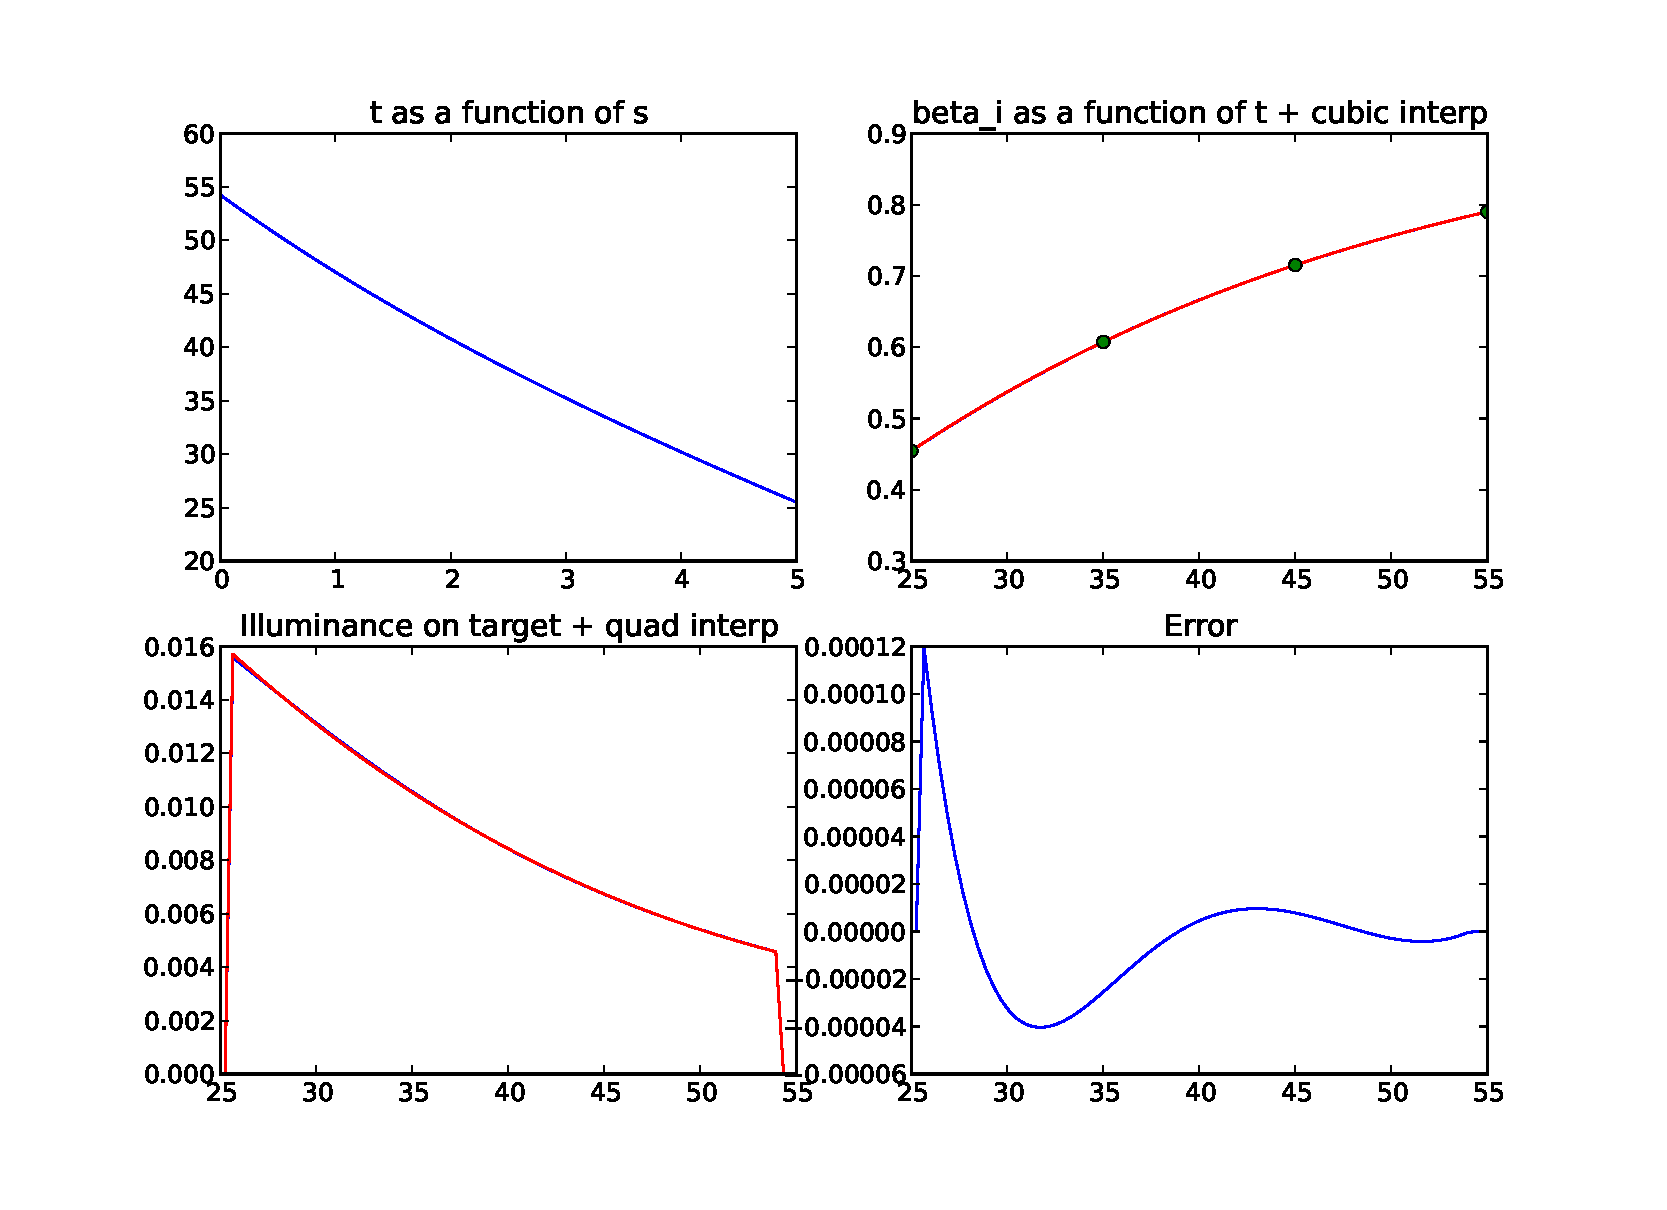
\includegraphics[scale=0.6]{linesrc_2d_ex} 
\caption{Target illuminance and quadratic fit for one surface
element.}
\label{fig:irr_one_element}
\end{figure}

\subsubsection*{Total light flux (computation from Gideon)}
Let the optical surface be delimited by two fixed 
points $p_1(x_1, y_1)$ at the bottom and $p_2(x_2, y_2)$ at the top.
The total light flux emitted by the source and reaching the surface needs
to be computed to ensure a unit source power.
This writes:
\begin{equation}
\label{eq:power_scale}
 \Phi_S  
= \int_{s_{min}}^{s_{max}} \int_{\beta_{min}(s)}^{\beta_{max}(s)} 
     L_S(s,\beta_i)ds\,d\beta_i
\end{equation}
where the boundaries of the inner integral are functions of $s$:
\[ \beta_{min} = \tan^{-1}\left(\frac{y_1-s}{x_1}\right) \quad\quad 
   \beta_{max} = \tan^{-1}\left(\frac{y_2-s}{x_2}\right)\]

The simple case of a Lambert uniform source (no dependence on $s$) can be computed 
analytically:
\[ \Phi_S  
= \int_{s_{min}}^{s_{max}} \int_{\beta_{min}}^{\beta_{max}} 
      \cos\beta_i\,ds\,d\beta_i = \int (\sin\beta_{max} - \sin\beta_{min})ds
 = F(s_2) - F(s_1)
    \]
\[  \quad\text{with}\quad
  F(s) = \sqrt{x_2^2  + (s-y_2)^2} - \sqrt{x_1^2  + (s-y_1)^2} \]

In practice a super Gauss function is used to delimit the extent of the source
in order to avoid numerical instabilities when discretizing the surface.
The computation above is then slightly off. This is corrected by computing
numerically the total source light flux falling on the target (considering
an extended target to capture all the rays), and scaling the source power
by this factor.

\subsubsection*{Luminance transformation through a circular interface}
Supposing that the extented source is covered by a spherical optical interface,
we look for the virtual source luminance that is seen by the rest of the 
system. The source plane is immersed in a medium $n_1$, the part on the right
of the (blue) optical surface is immersed in $n_2$.
The Fig.~\ref{fig:virt_lum} below presents the notations used in this section and
represents a ray being diffracted (with $n_1 > n_2$).

\begin{figure}[!htbp]
\centering
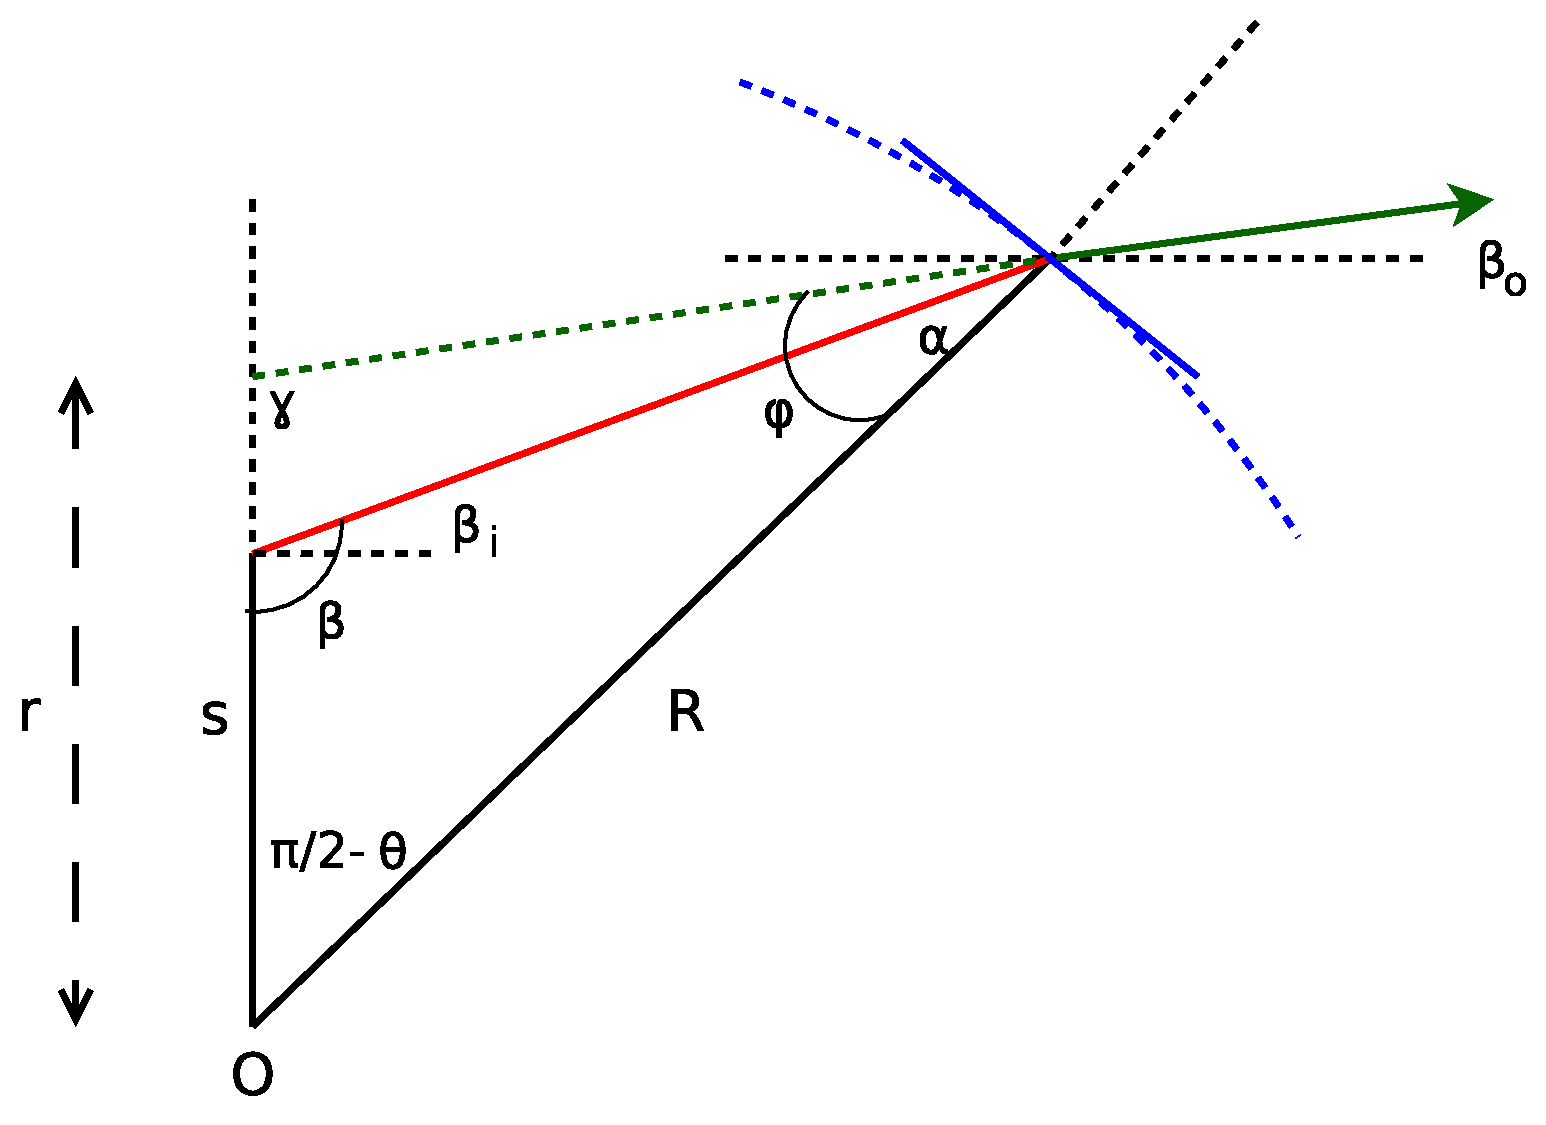
\includegraphics[width=0.6\textwidth]{virt_luminance} 
\caption{Computation of the virtual luminance produced by a spherical interface (in blue).
Incoming ray in red, output ray in green (emitted virtually from the coordinate $(0, r)$
with an angle $\beta_o$).}
\label{fig:virt_lum}
\end{figure}

We now look for the transformation $F: (r, \beta_o) \mapsto (s, \beta_i)$, the bijection
associating a single ray from the new virtual source (as produced by the spherical optics)
 to a single ray of the real source.

The sine law in the triangle with left side $r$ writes:
\[ \frac{\sin\phi}{r} = \frac{\sin\gamma}{R}\]
The angle relationships are:
\[ \beta = \pi/2+\beta_i  \quad\textrm{and}\quad  \gamma = \pi/2 + \beta_o\]
\[ \phi = \pi - \gamma - (\pi/2 -\theta) = \theta - \beta_o \]
\[\beta_i + \alpha = \theta \]
Hence:
\[ \sin\phi = r\frac{\sin\gamma}{R} = r \frac{\cos\beta_o}{R} \]
and
\begin{equation}  
 \theta = \beta_o + \arcsin\left( \frac{r}{R}\cos\beta_o\right)
 \label{eq:lum_theta}
\end{equation}
Snell's law writes: $n_1 \sin\alpha = n_2\sin\phi$ yielding:
\begin{equation}  
\alpha = \arcsin\left( \frac{n_2 r}{n_1 R}\cos\beta_o \right)
 \label{eq:lum_alpha}
\end{equation}

We thus obtain the first part of the coordinate transform:
\begin{equation}
\beta_i = \theta-\alpha = \beta_o + \arcsin\left( \frac{r}{R}\cos\beta_o\right)
                         - \arcsin\left( \frac{n_2 r}{n_1 R}\cos\beta_o \right)
\label{eq:lum_betai}
\end{equation}

Similarly in the smaller triangle with $s$ as left side, the sine law writes:
\[  \frac{R}{\sin\beta} = \frac{s}{\sin\alpha} \]
yielding:
\begin{equation}
 s = R\frac{\sin\alpha}{\sin\beta} = R\frac{\sin\alpha}{\cos\beta_i}
%   =  r\frac{n_2}{n_1}\frac{\cos\beta_o}{\cos\beta_i}
 \label{eq:lum_s}
\end{equation}

We note that if $n_1=n_2$, the equations \eqref{eq:lum_betai} and \eqref{eq:lum_s} 
gives back as expected the original coordinates of the virtual source.
 The Jacobian of $F$ will be needed, and involves derivating~\eqref{eq:lum_theta} and
\eqref{eq:lum_alpha} with respect to $r$ and~$\beta_o$.
We then have:
\[
\pderiv{\theta}{r}  = \frac{\cos\beta_o}{R} \frac{1}{\sqrt{1-\sin^2\phi}}
      =  \frac{\cos\beta_o}{R \cos\phi}
 \quad  \quad \textrm{and} \quad  \quad 
\pderiv{\theta}{\beta_o}  =  1- \frac{r}{R}\sin\beta_o \frac{1}{\sqrt{1-\sin^2\phi}}
        =  1- \frac{r}{R} \frac{\sin\beta_o}{\cos\phi} \\        
\] \[
\pderiv{\alpha}{r}  = \frac{n_2}{n_1}\frac{\cos\beta_o}{R}\frac{1}{\sqrt{1-\sin^2\alpha}}
        = \frac{n_2}{n_1}\frac{\cos\beta_o}{R\cos\alpha}
 \quad \textrm{and} \quad
\pderiv{\alpha}{\beta_o} = -\frac{n_2 r}{n_1 R}\sin\beta_o\frac{1}{\sqrt{1-\sin^2\alpha}}
        =  -\frac{n_2 r}{n_1 R}\frac{\sin\beta_o}{\cos\alpha}
\]

The partial derivatives $\pderivi{\beta_i}{r}$ and $\pderivi{\beta_i}{\beta_o}$ are
readily computed from the difference expressed in~\eqref{eq:lum_betai}.

A bit more work is required for $s$: we write its total differential with respect to the 
two angle variables involved in~\eqref{eq:lum_s} and use the chain rule:
\[ ds = \pderiv{s}{\alpha}d\alpha + \pderiv{s}{\beta_i}d\beta_i \]
With:
\[
d\alpha = \pderiv{\alpha}{r}dr + \pderiv{\alpha}{\beta_o}d\beta_o
\quad\textrm{and}\quad
 d\beta_i = \left(\pderiv{\theta}{r} - \pderiv{\alpha}{r}\right) dr + 
        \left(\pderiv{\theta}{\beta_o} - \pderiv{\alpha}{\beta_o}\right) d\beta_o
 \]
we can write:
\[ds =  \left[ \pderiv{s}{\alpha}\pderiv{\alpha}{r} 
             + \pderiv{s}{\beta_i}\left( \pderiv{\theta}{r} - \pderiv{\alpha}{r} \right)
        \right] dr 
+       \left[ \pderiv{s}{\alpha}\pderiv{\alpha}{\beta_o} 
             + \pderiv{s}{\beta_i}\left( \pderiv{\theta}{\beta_o} - \pderiv{\alpha}{\beta_o} \right)
        \right] d\beta_o\]
We can compute:
\[ \pderiv{s}{\alpha} = R\frac{\cos\alpha}{\cos\beta_i} 
   \quad\textrm{and}\quad  
   \pderiv{s}{\beta_i} = R\frac{\sin\alpha}{\cos\beta_i}\tan\beta_i
   \] 
and thus the final partial derivatives as function of $r$, $\beta_o$ and the four
partial derivatives expressed previously:
\[\pderiv{s}{r}  = \frac{R}{\cos\beta_i}  \left[
      \cos\alpha\pderiv{\alpha}{r} + \sin\alpha\tan\beta_i
             \left( \pderiv{\theta}{r} - \pderiv{\alpha}{r} \right) 
    \right]
\]
\[
\pderiv{s}{\beta_o}  = \frac{R}{\cos\beta_i}  \left[
      \cos\alpha\pderiv{\alpha}{\beta_o} + \sin\alpha\tan\beta_i
            \left( \pderiv{\theta}{\beta_o} - \pderiv{\alpha}{\beta_o} \right)
     \right]
\]

The final Jacobian of $F$ is written:
\begin{equation}
J_\Phi = \pderiv{s}{r}\pderiv{\beta_i}{\beta_o} - \pderiv{\beta_i}{r}\pderiv{s}{\beta_o}
\end{equation}
and numerically the following intermediate values are computed: $\alpha, \phi, \theta $
 plus the four partial
derivatives of $\theta$ and $\alpha$ with respect to $r$ and $\beta_o$.

We can now conclude with a similar reasoning as what has been done previously. The 
elementary light flux from the real source writes:
\[d^2\Phi_S = L_S(s, \beta_i)\,ds\,d\beta_i\] 
and is equal to the elementary light flux from the virtual source:
\[ d^2\Phi_V = L_V(r, \beta_o)\,dr\,d\beta_o\]
With the change of variable $F$ one has direclty the virtual luminance as a function
of the real one:
\begin{equation}
L_V(r, \beta_o) = L_S(s, \beta_i) |J_F|
\end{equation}

Figure~\ref{fig:virt_lum_all} shows an example of the luminance transformation for a 
Lambert source and for an isotropic source.
The start luminance for an isotropic source is not represented as this is simply
a constant value across the square phase-space domain.
Without surprise and as can be seen with the Jacobian on~Fig.~\ref{fig:virt_lum_fred}
most of the distortion effect happens at the extreme points of the phase-space (extreme
emission angles, or source boudaries).

\begin{figure}[!htbp]
\centering
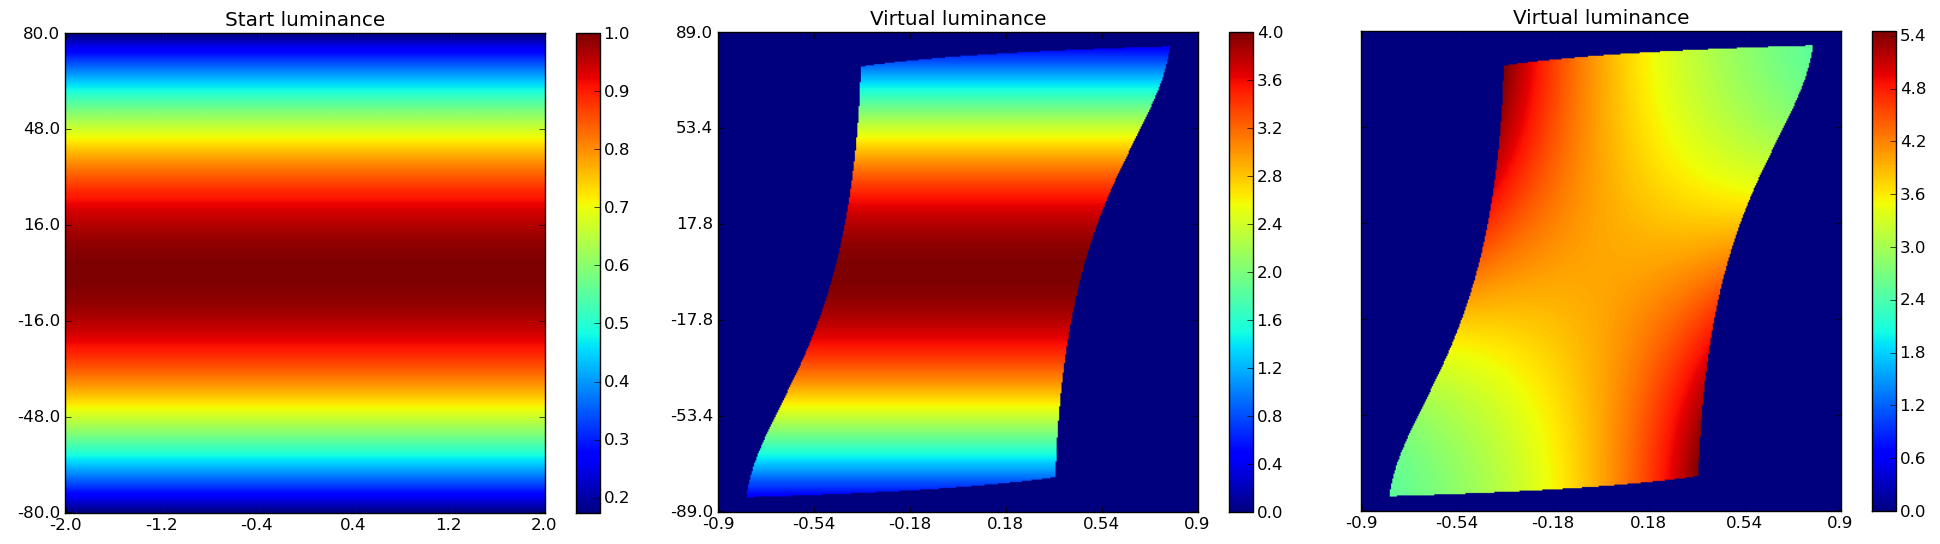
\includegraphics[width=1.0\textwidth]{virt_lum_ALL} 
\caption{Luminance source transformation - phase space representation (space coordinate
on the x axis in $mm$, angle coordinate in degrees). \textit{Left to right}: 
(a) Lambert source luminance; (b) Virtual luminance through the optics (Lambert source);
(c) Virtual luminance through the optics (Isotropic source).}
\label{fig:virt_lum_all}
\end{figure}

The virtual light irradiance (resp. intensity) can be computed from the phase space
function by integrating along the angle coordinate (resp. space coordinate). Both the
resultin irradiance and resulting intensity can be ray-traced with FRED. The figure~
\ref{fig:virt_lum_fred} shows a very good agreement. 
The simulation and computation was performed with a somewhat extreme setup (isotropic
source, source half-extent of $2\,mm$ and sphere radius of $4\,mm$, material index
$n_2 = 4$). Even with this, we see that the effect of the Jacobian is minimal, especially
on the irradiance distribution.

\begin{figure}[!htbp]
\centering
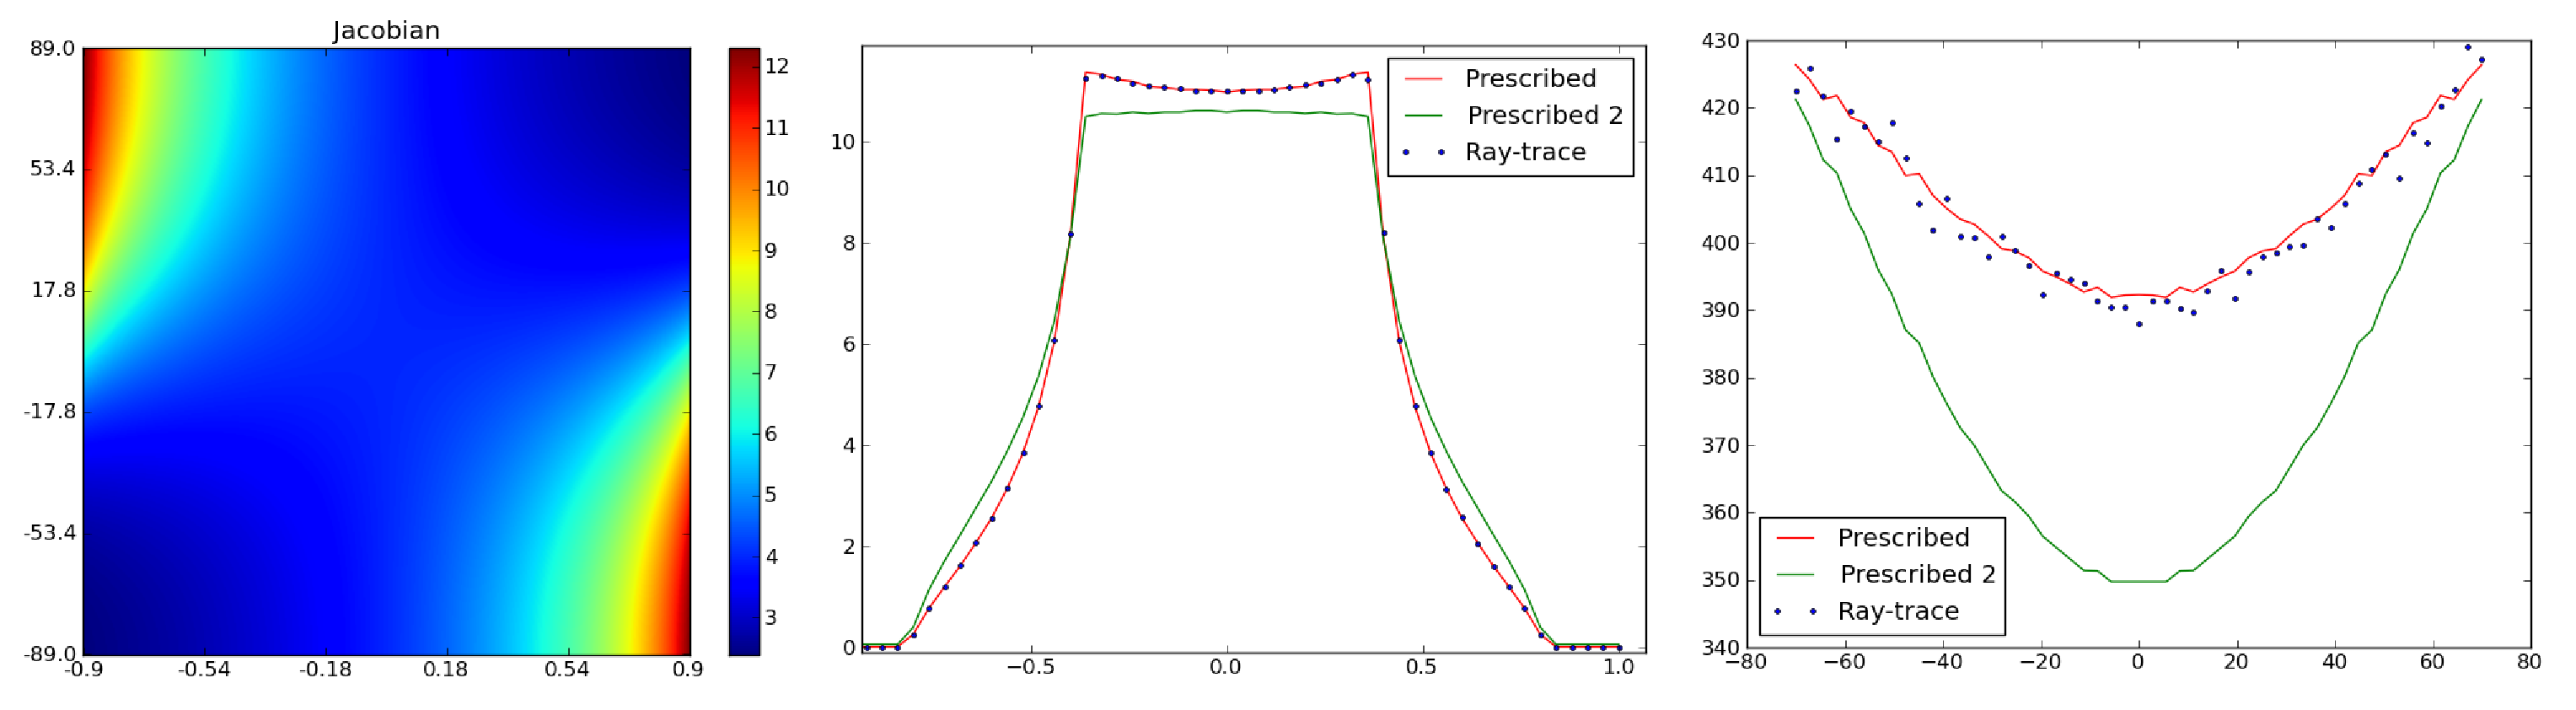
\includegraphics[width=1.0\textwidth]{virt_lum_FRED} 
\caption{(a) Jacobian of the Luminance transform (same axis as previous figure)
(b) FRED ray-tracing and \textit{irradiance} comparison. 
 With Jacobian factor in red, without (and scaled appropriately) in green; 
 (c) Same thing for the \textit{intensity}. }
\label{fig:virt_lum_fred}
\end{figure}

We also note that the total power is indeed conserved: when integrating the whole phase
space area, the start luminance and the virtual luminance amouts to the same total
light power (relative error below 0.6\% for a resolution of $400\times 400$ and diminishing
linearly with the resolution).

All in all the main effect of the spherical optics for normal conditions is to provide
a smaller apparent source (when $n_2 > n_1$). The irradiance and 
intensity distribution retain a very similar form
to what the original source provides (i.e. with no spherical optics).

\subsubsection*{Numerical results}
The points above allow to perform an optimization to realise a given irradiance.
The target area is discretized and at each point a comparison is made between 
the prescribed irradiance and the irradiance computed via \eqref{eq:computed_irr}.

The appropriate power scaling doesn't rely in practice on \eqref{eq:power_scale}
for various reasons: a) the irradiance produce by a face alone may mathematically
become negative in eq XXX - this corresponds to a physical situation where
TIR occurs. 
b) the intensity emitted by a point in the source plane is not implemented with
a true sharp cut-off, but instead with a super-Gauss function to avoid numerical
noise due to the surface discretization (TODO enhance this explanation).

Practically the total power from the source is simply assessed by integrating the overall
computed irradiance on a somewhat larger target.

\textbf{TODO write more here - SPIE Barcelona 2012}

\begin{figure}[!htbp]
\centering
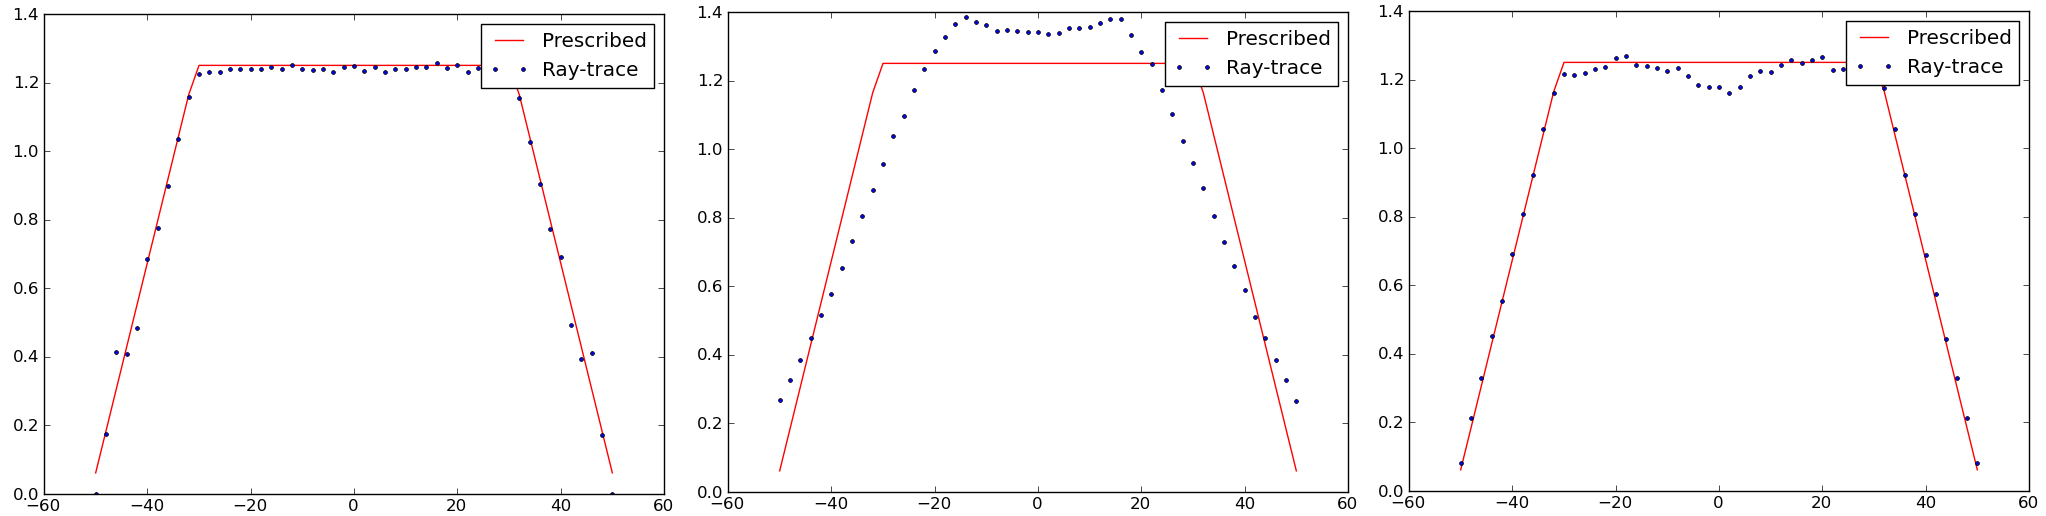
\includegraphics[width=1.0\textwidth]{fred_ww} 
\caption{Point source / Extended source =2mm (no optim) / Extended source optimized. }
\label{fig:res_fred_ww}
\end{figure}

\begin{figure}[!htbp]
\centering
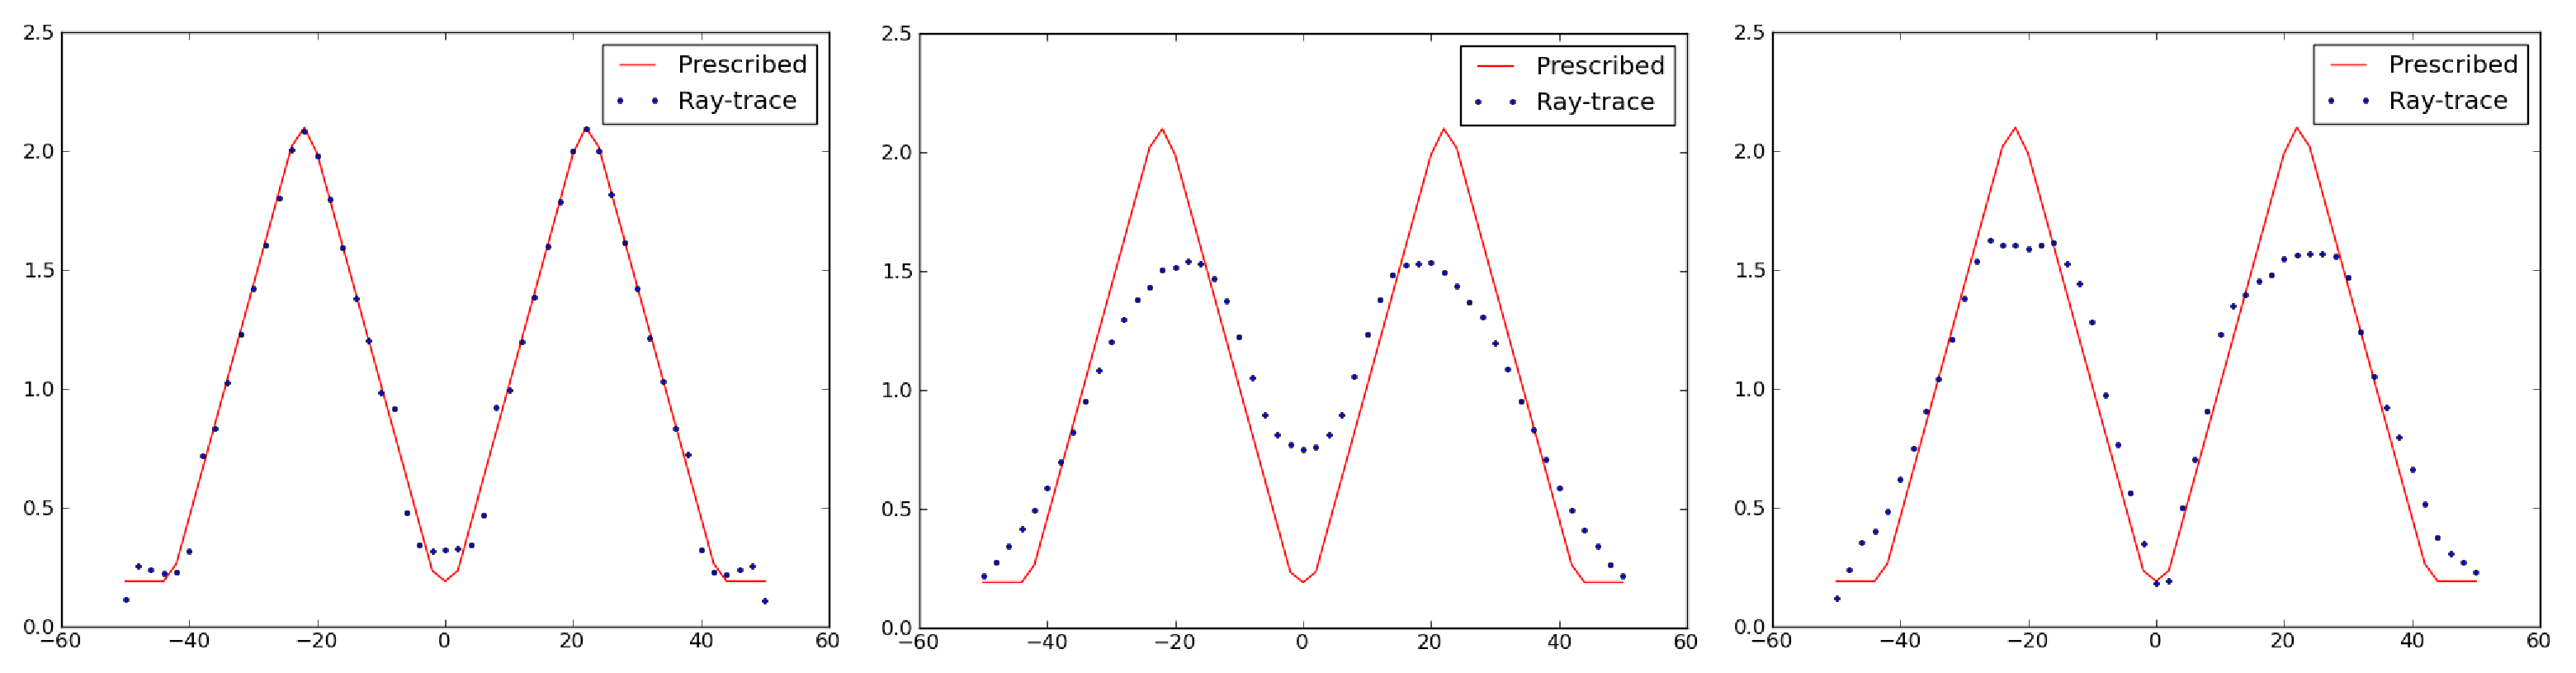
\includegraphics[width=1.0\textwidth]{fred_ring} 
\caption{Point source / Extended source (no optim) / Extended source optimized. }
\label{fig:res_fred_ring}
\end{figure}

\begin{figure}[!htbp]
\centering
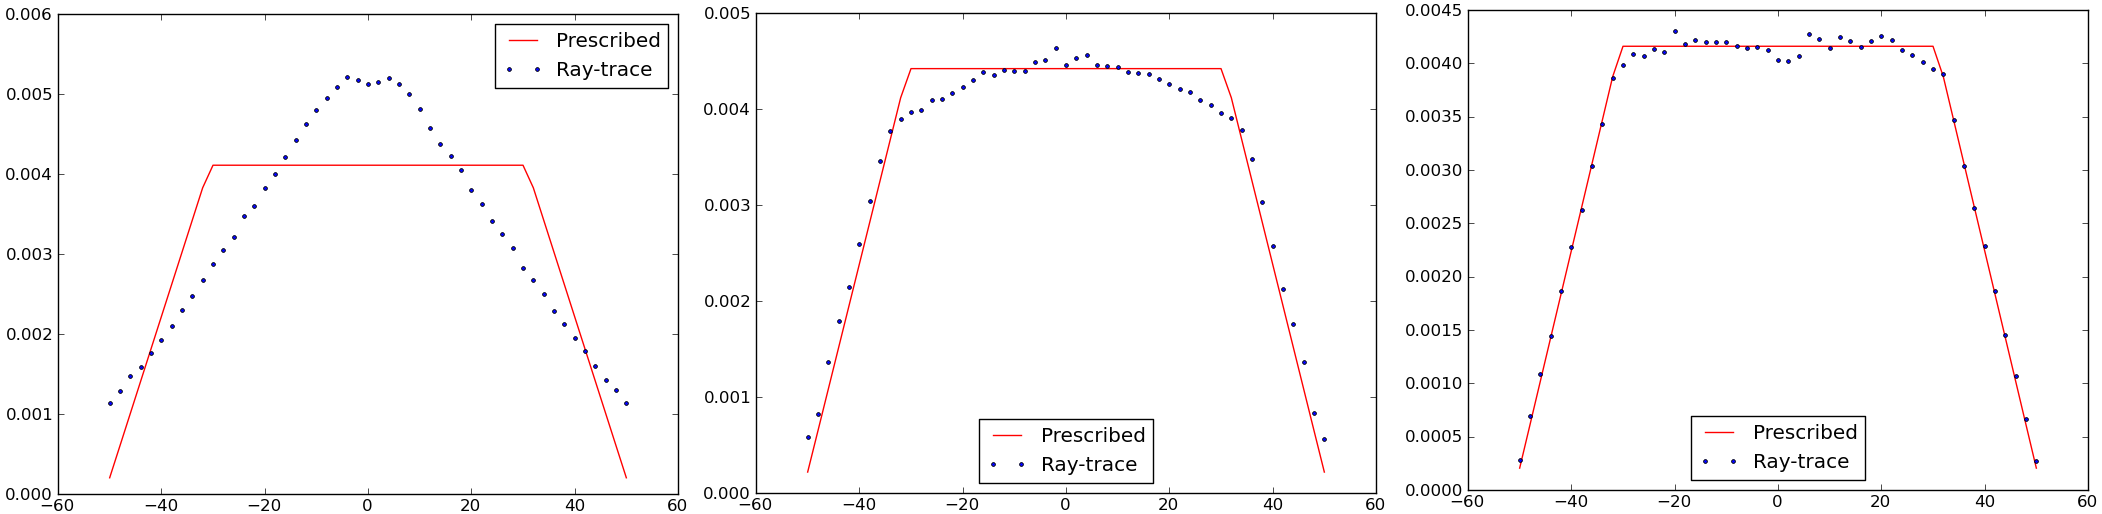
\includegraphics[width=1.0\textwidth]{fred_ww_withsphere} 
\caption{ Source = 3mm: a) one surf no optim b) one surf optim c) with spherical optics R=3mm}
\label{fig:res_fred_ww_sphere}
\end{figure}

\begin{figure}[!htbp]
\centering
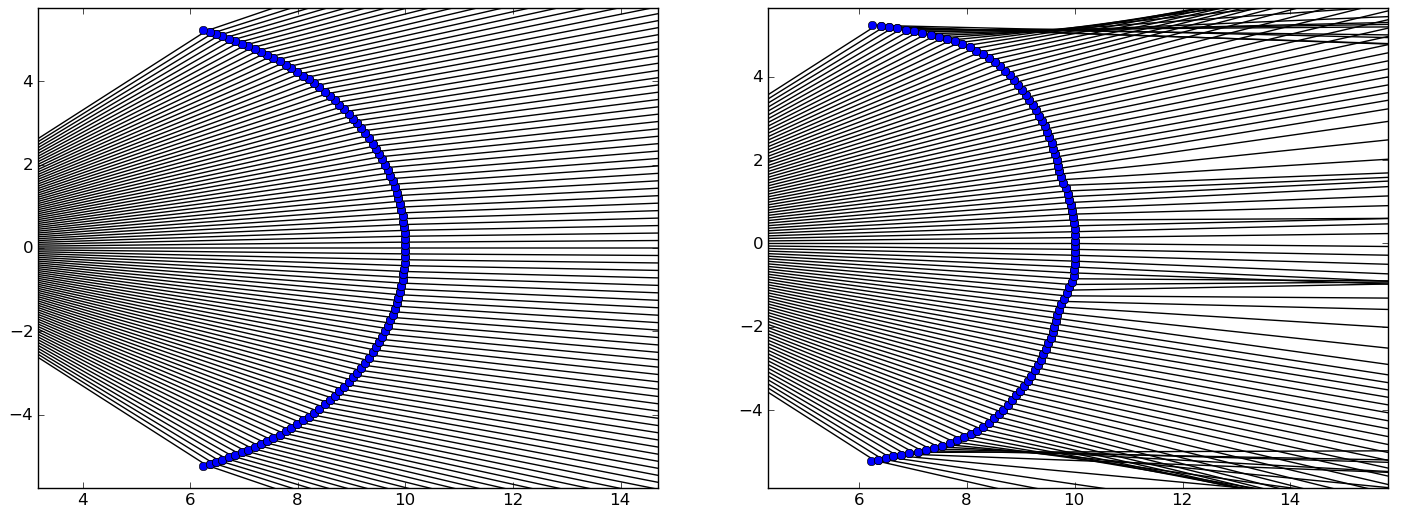
\includegraphics[width=1.0\textwidth]{ww_surfaces} 
\caption{WW - Point source ray tracing - a) Surface for point source / Surface for ext source}
\label{fig:res_ww_surfaces}
\end{figure}

\subsection{Three dimensional case - Elementary surface element \red{TODO rewrite}}
The reasoning is very similar in 3D but the full computation
of the previous differential element is painful.
The implemented algorithm already allows to compute
the image of a source point onto the target.
This can be fitted quadratically using techiques similar to what
is done in FEM (see Rolf's implementation IsoparFEM2D).

The source is parametrized by the coordinates $(r, s)$ and
the target by $(X, Y)$. A given source ray hitting the surface
element located at $P(\alpha, \beta, \gamma)$ has spherical 
directions $(\theta, \phi)$.

The energy conservation writes:
\[ I(\theta, \phi, r, s)d^2\Omega = B_t(X, Y)dXdY\]
with $I$ the source intensity, $d^2\Omega = d\theta d\phi\sin(\theta)$
 the solid angle 
seen by the surface element in the direction of 
the source, and $B_t$ the irradiance
on the target.

With two changes of variable, this can be rewritten into:
\[ B_t(X, Y)dXdY = I(\theta, \phi, r, s)|J_1| 
\sin(\theta) dr ds  \]
\[ B_t(X, Y)dXdY = I(\theta, \phi, r, s)|J_1|. |J_2| \sin(\theta) dX dY\]
\[ B_t(X, Y) = I(\theta, \phi, r, s)|J_1|. |J_2| \sin(\theta)\]
with $J_1$ the Jacobian of the transformation 
$(r, s) \mapsto (\theta, \phi)$ and $J_2$ the Jacobian of the 
transformation $(X, Y) \mapsto (r, s)$. The (inverse of the) 
latter is evaluated
numerically thanks to the quadratic fit.

Let's compute $J_1$.
The light incident vector on the surface element is 
$\mathbf{I}(\alpha-r, \beta-s, \gamma)$.
 The Cartesian to spherical 
coordinate transformation formulas write:
\[ R = \sqrt{(\alpha-r)^2+(\beta-s)^2+\gamma} \]
\[ \phi = \arctan(\frac{\beta-s}{\alpha-r}) \]
\[ \theta = \arccos(\gamma/R) \]
Differentiating:
\[ dR = -\frac{(\alpha-r)dr + (\beta-s)ds}{R} \]
\[ d\theta = \frac{\gamma dR}{R^2 \sqrt{1-(\gamma/R)^2}} 
 = -\frac{\gamma}{R^3} \frac{(\alpha-r)dr + (\beta-s)ds}
{\sqrt{1-(\gamma/R)^2}} \]
With a simple trigonometric transformation one also readily
obtains:
\[ sin(\theta) = \sqrt{1-(\gamma/R)^2} \]
hence:
\[ \sin(\theta) d\theta = 
 -\frac{\gamma}{R^3} \left[ (\alpha-r)dr + (\beta-s)ds \right] \]
Similarly
\[ d\phi = d\left(\arctan\frac{\beta-s}{\alpha-r} \right) 
= - \frac{(\alpha-r)ds - (\beta-s)dr}{(\alpha-r)^2 + (\beta-s)^2}
\]
Finally one obtains for the Jacobian times the sine an 
impressive cancellation of terms:
\[ \sin(\theta) J_1 = \sin(\theta)\left( \pderiv{\theta}{s} 
\pderiv{\phi}{r} - \pderiv{\phi}{s}\pderiv{\theta}{r} \right) 
 = -\frac{\gamma}{R^3}\]

(TODO: could be seen with a physical argument stating that
this quantity doesn't depend on the azimuth $\phi$).

This has been validated in FRED:



% 
\chapter{Segmented optics ??}

\chapter{Conclusion}
\label{ch:conclu}
Blabla extended source is a real challenge


% Appendix 
%\chapter*{Appendix}
\label{ch:appendix}

\section*{Vector calculus identities}

\section*{Photometric and radiometric units}

\section*{Lambert source power}

% Bibliography


\end{document}